\documentclass{l4proj}


\usepackage{url}
\usepackage{amssymb}
\usepackage{graphicx}
\usepackage{algorithmic}
\usepackage[ruled,vlined]{algorithm2e}
\usepackage{amsthm}
\usepackage[ampersand]{easylist}
\usepackage{subcaption}

\newtheorem{thm}{Theorem}
\newtheorem{definition}{Definition}
\newtheorem{lemma}{Lemma}
\setcounter{secnumdepth}{5}
\setcounter{tocdepth}{5}

\begin{document}
\title{In-Car Gestural Interaction}
\author{Gerard Romeo}
\date{March 28, 2014}
\maketitle

\begin{abstract}
\end{abstract}

\educationalconsent
%
%NOTE: if you include the educationalconsent (above) and your project is graded an A then
%      it may be entered in the CS Hall of Fame
%
\tableofcontents
%==============================================================================

\chapter{Introduction}
\pagenumbering{arabic}
\label{sec:intro}
\vspace{-3mm}
As technology progresses, car manufacturing companies are consistently looking for ways to integrate these systems into their new designs in innovative ways. However, such advancements bring safety concerns; if the device is located in an inconvenient location for the driver, attempting to use the device could hamper and detract the driver’s attention, thus potentially leading to accidents.

This has led to a deep pool of research analysing how to improve interaction within automotive UI. Various forms of multimodal techniques have been implemented within the interior of vehicles successfully. With the emergence of recent free-gestural motion technology that can accurately determine a user's gesture, the field of Human Computer Interaction (HCI) is pursuing ways in which this could be adapted into the automotive industry. This is especially prevalent considering that research has shown[1] that gestural input maintains a driver’s awareness and perception on the road, whilst haptic inputs, such as buttons can provide an additional layer of potential distraction.  

Gestures and body language are an integral part of societal interaction -- they are natural subconscious reactions that are complimentary to speech. They provide a visual representation of what is being communicated. They allow a form of communication when language becomes a barrier - there are signals that within society feel pre-defined and are instantly recognisable. In cultural anthropology, human body language is the primary contributor to non-verbal communication studies and gestures are often used throughout all cultures. With this in mind I would like to propose using some of these widely accepted gestures to interact with a variety of the vehicle's interior functionality. 

The aim of my project, titled {\it In-Car Gestural Interaction}, is to create a series of quick, intuitive gestures that will allow drivers to interact with systems within their car, providing an alternative form of modality that the typical haptic buttons found in modern day vehicles provide. 

Furthermore, as previous research indicates, this should prevent the driver’s focus from deviating from the road.  Therefore, not only will the development of the gestures provide a useful alternative for drivers, it also has the potential to improve road safety, ultimately leading to less accidents and deaths as a result. 

{\it In-Car Gestural Interaction} aims to provide a novel and alternative way of interacting with an automobile’s multimedia devices and interfaces. Such gestural interaction should complementary to the driver, improving their awareness on the road with the hope of reducing distractions and improving the safety of the road. 


\chapter{Background and Related Work}
\label{sec:back}
\vspace{-3mm}
\section{Motivation}
\vspace{-3mm}
In recent years there has been a sudden influx of free-motion gestural technologies that have opened up new horizons in the automotive industry. Car manufactures such as Hyundai and BMW have invested Research and Development into developing concept designs that seamlessly integrate the use of gestures with the motion detection capabilities built into the steering wheel. However, these concepts only use simple gestures such as swiping to navigate hierarchical menus and still require the driver to focus on the central display built into the hub of their car.

Furthermore, free-motion gestural interaction within vehicles has been studied throughout the years. Although the technology has never been reliable to apply in real-world scenarios, their findings from controlled-environment experiments highly suggest that hand gestures could be the optimal form of interaction within automobiles.

This section will consider the pre-existing background research, the current state of gesture controls within the automotive industry and discuss why gesture based interaction could potentially be the safest input modality whilst driving.  

\section{What is Gesture Recognition?}
\vspace{-3mm}
Gesture Recognition in Computing Science is the study of understanding and responding to human movement. Gesture and body language can exist from any part of the body but is most commonly recognised as hand of facial movements, often stemming from emotional responses. 

As technology has progressed, so to has our ability to read and interpret these gestures through a series of algorithms. Particularly, Computer Vision is the experimental field that strives to improve the way in which we acquire, process, analyse and understand real-life high-fidelity data in order to produce numerical or symbolic information. With this improvement in Computer Vision, it is now possible to recognise and more importantly, respond to a user's emotions and gestures.

The belief is that with a greater understanding of human body language and gestural interaction, the world of Human Computer Interaction (HCI) will evolve to the state that we are no longer reliant on on input devices such as a keyboard and mouse, but instead users can control devices through Gesture Recognition. 

\section{Gesture Recognition Devices}
\vspace{-3mm}
Gesture technology is typically in the field of research and development and as a result, the technology ultimately becomes overtly expensive, specifically built for one purpose and is never released to public. However the following two devices have not only been released to the masses but are relatively inexpensive, providing future avenues for the adoption of gesture recognition. 
\subsection{Microsoft Kinect}
\vspace{-3mm}
When Microsoft released its Kinect peripheral in 2010 it revitalised the concept of free-motion gestural interaction. No longer did users have to interact with an input device -- the Kinect could determine a person's actions and body movements, allowing the user to interact without any other form of input peripheral. This is considered by many to be the first time that full body gestural movements had garnered such public acceptance. The Kinect is not without its technical caveats however.
\begin{figure}[h!]
\centering
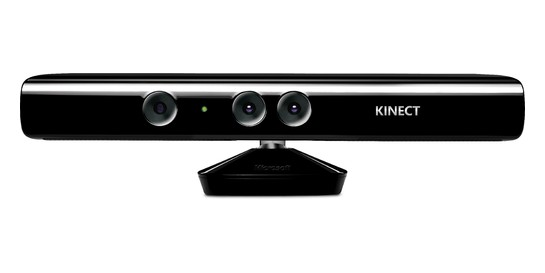
\includegraphics[width=4in]{images/kinect.jpg}
\caption{Microsoft Kinect Peripheral}
\label{fig:kinect}
\end{figure}

The Kinect operates by sending out infrared beams from the emitter on its base and the reflected beams are then read by the infrared depth sensor. The time delta’s between these reflected beams is then used to interpret the depth of field in the area and the distance between the Kinect and objects within its field of view, such as a human. The device then uses skeletal tracking to create a 3D structure of the person and recognise their limbs, hence allowing gestures to be defined within its field of view.

\subsection{LeapMotion}
\vspace{-3mm}
In 2012 the LeapMotion Controller was released to public, aiming to provide a much higher fidelity and accuracy for finger tracking. As the LeapMotion is capable of tracking all 10 fingers up to 1/100th of a millimeter, it has provided new and unparalleled avenues in gesture recognition.
\begin{figure}[h!]
\centering
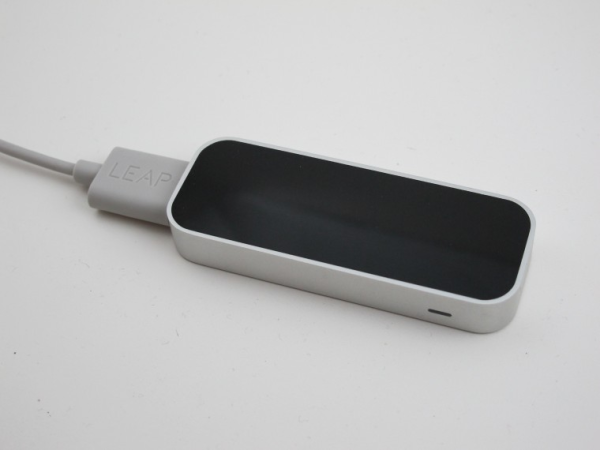
\includegraphics[width=3in]{images/leap.png}
\caption{LeapMotion Device}
\label{fig:leap}
\end{figure}

With a 150° field of vision and 3-Dimensional depth tracking, a users hand can be measured with extreme accuracy. Using two monochromatic infrared cameras and three infrared LEDs, the LeapMotion observes an approximation of a hemispherical area, at a distance of about 1 meter. The LEDs generate a 3D pattern of dots of IR light[14] and the reflected information returns to the device at around 200 frames per second. This data is then analysed and processed by the Leap Motion's patented algorithms to then synthesise a hand and its appendages 3D positional data by comparing the 2D frames generated by the two monochromatic cameras.

As it offers an unprecedented level of precision, it is the most sensitive gestural technology to date.

\section{Related Research}
\vspace{-3mm}
In-car Gestural Interaction is not a new concept within the automotive industry, but it has yet to be established commercially and lacks the credence of other input modalities. Since the dawn of gestural technology, automotive designers and researchers have attempted to integrate gestural input recognition into vehicles. The especially became relevant when periphery multimedia devices were incorporated into cars, know as vehicle telematics. Developers and car manufacturers have experimented a number of input modalities, seeking to obtain the safest, most practical option for drivers. However, a lack of consensus existed as to what input modality would be the most suitable to control such gadgets. 

As technology within vehicles has improved and expanded, this has enforced an increased need for functionality and haptic controls to be built into the vehicle's dashboard or steering wheel. 

\subsection{Previous Research}
\vspace{-3mm}
In 2001, the Institute of Human Machine Communication at the Technological University of Munich \cite{}suggested an alternative to haptic controls would be required as the number of physical controls in vehicles were becoming increasingly confusing and demanding on drivers. They proposed using hand gestures to simplify user interaction. This was carried out by creating a defined gesture space to the right of the steering wheel -- note that as this experiment took place in Munich, Germany, where vehicles are left hand drive. As such, the `driver' in the experiment carried out gestures with his right hand, towards the center of the car's interior. 

The experiment was carried out in a controlled environment and by allowing participants to explore gestures for specific scenarios, they discovered that certain gestures were culturally independent, such as a mimicking action for answering a phone-call. Such gestures would not have to be learned as they synonymous within society.

However, through experimentation they also discovered that users were only able to recall a small portion of the gesture library and that participants were unsure of which gestures to use in given scenarios, presenting a lack of gesture-conformity. This was overcome by developing a help notification system in the vehicle's User Interface (UI), to develop users learning curve. Given users low threshold to identify gestures it was noted that without an optimization of gesture libraries and their ease of recognition, gestures within vehicles would provide a further layer of distraction. Users would be reliant upon the UI visualisation and not the gestures themselves, resulting in user annoyance. Despite these issues, the study suggested that gestures are a viable multimodal method for in-car interaction, given that the gestures had high-conformity with users.

This research was further analysed by Alpern and Minardo \cite{}, whose study looked at developing a car gesture interface to control secondary tasks. Driving is a cognitively demanding task, requiring the attentiveness of the driver at all times. After iterating through several UI techniques, such as hierarchical menus and virtual objects, Alpern and Minardo developed a heads-up display interface that integrated over the driver's HUD. Gestures were limited to simple swipes and counts based on the number of fingers shown on a given hand. 

From their experimental results, they found that the gesture interface for the radio was not only comparable to the haptic radio alternative, that can be found in every car, but that it also increased the driver's attentiveness on the road. This was due to the simple gestures implemented and that the interface could be quickly glanced at whilst still focusing on the road, permitting the driver to be aware of potential hazards.

Although both research papers offer critical praise for gestural interaction within vehicles, neither were able to apply their systems in real world scenarios. The experimental evaluation methodology was a result of the limitations of gesture detecting hardware. 

The technology used approximately 10 years ago was impractical and inaccurate to be tested out with experimental findings; as the hardware used was based upon infrared depth cameras, they would be affected by the varying light conditions that drivers will experience. The infrared cameras used to detect the gestures were unable to compensate between the day/night cycle and as such, were not stable and reliable for commercial applications. 

The evidence found in these findings however suggested a direct correlation between gestural interaction and the stability of the driver's road awareness.

\subsection{Current Research}
\vspace{-3mm}
In recent years, there has been an influx of gesture recognition peripherals that have revitalised the automobile industries interest in gestures as an input modality. Now that the devices are much more stable and reliable, they can be used to control the plethora of {\it`infotainment'} functions that vehicles currently have at their disposal. 

With this resurgence of free-motion gestures, new research has been carried out and with the improvement accuracy, they have been able to retrieve more conclusive findings as improved recognition and reliability permits real world field testing. 

In a recent study, Loehmann \textit{et al.} \cite{} were able to conclude that ``gestural interaction strengthens attractiveness and hedonic quality significantly compared to haptic interaction'' and that from their 20 participants that carried out their test, ``14 favoured the gestures''[5]. This qualitative data was retrieved 
In addition to this, they also considered what gestures can be viewed as socially and culturally independent, with the aim of minimalising the number of gestures that would be recognised through the device, citing that redundancy of gestures could lead to confusion. They concluded that further work would be required for commercial gestural products. 

TO DO!!!

\section{Examples In Automotive Industry}
\vspace{-3mm}
The first instance and sign that gestural interaction would come to the forefront of the Automotive Industry was with BMW's commercial release of its contactless tailgate opening system[3], which would allow passengers to open the trunk of their car by performing a foot gesture below the rear bumper, permitting they held the key in their possession. This feature has been advertised strongly in models that have implemented the technology and holds many use-cases, such as returning to the vehicle with a number of bags or luggage in your possession. Instead of having to place the bags down, all the person has to do is motion their foot under the rear-side bumper. 
\begin{figure}[h!]
\centering
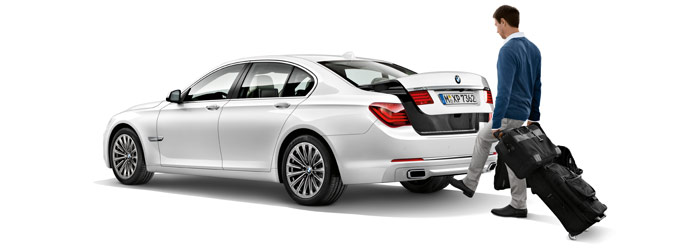
\includegraphics[width=4in]{images/contactless-tailgate.jpg}
\caption{Gentleman Showcasing BMW's Contactless Tailgate}
\label{fig:BMW}
\end{figure}

With successful targeted marketing BMW's novel concept has been well received and is a useful addition, simplifying a driver's daily tasks. Despite the success of this, gesture based features have yet to be integrated into the interior of a manufactured vehicle. 

Gestural interaction has often been considered in the industry as it can ease the consumers life as this example shows. However, as it is an emerging market, as of yet, gestures only exist in the interior of the conceptual cars.

Typically these kind features found in conceptual cars are too far-fetched to exist in commercial production vehicles, but as more car manufacturers are investing into gestural technologies, it would imply that both technology and society is ready for the next step in automotive innovation. 

\begin{figure}[h!]
\centering
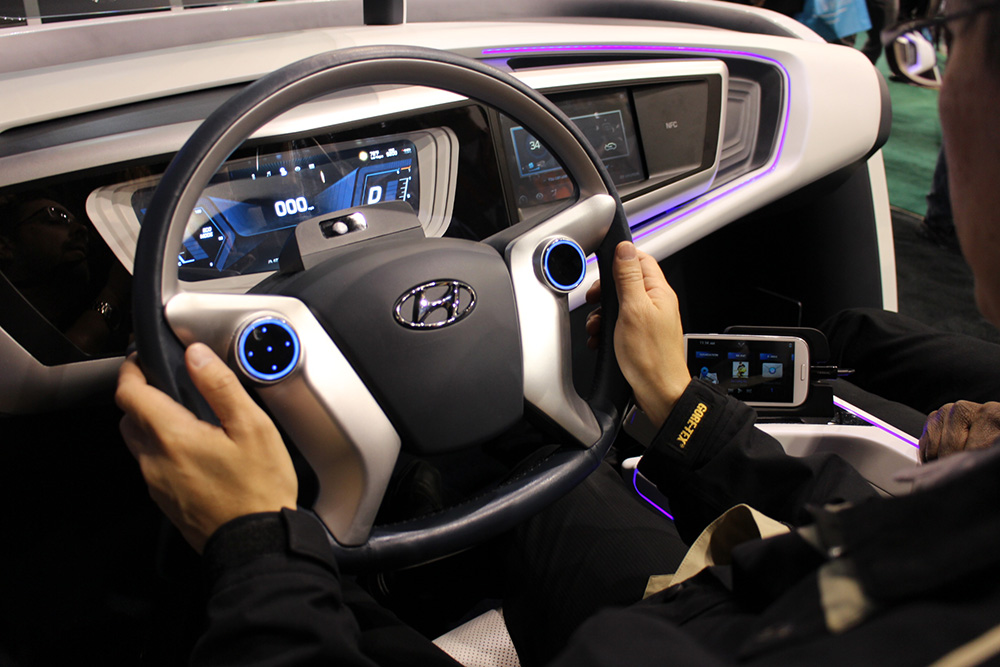
\includegraphics[width=4in]{images/hyundai.jpg}
\caption{Hyundai's `infotainment' steering wheel design}
\label{fig:hyundai}
\end{figure}

Hyundai\cite{} in particular have developed an `infotainment' concept car that adapts the steering wheel to have both haptic controls and gestural commands on the left and right hand side of the steering wheel respectively. These controls are used to interact with the vehicle's navigation systems, audio controls and other desirable functions. This allows for both physical and freehand control dependant on the driver's preference, as they are used to control the same features. \cite{}.

BMW have also forayed into this innovative form of HCI through a partnership with Harman, who are developing a new form of interface within vehicles that is primarily gesture-based\cite{}. As BMW have incorporate new features into their cars, so have the number of physical interactive elements -- modern cars can resemble aircraft cockpits; over-engineered to the point were new systems are underutilised due to the complexity of the design. BMW, recognising that the automotive market desires sleek, simple design, aim to allow users to control there systems with a small-set of simple gestures. The premise is similar to Hyundai but differs in the gesture recognition technology.

Kia also recently unveiled their User-Centered Driver (UCD) concept at the 2014 Consumer Electronics Show (CES 2014), that alongside an augmented reality display, incorporates gesture recognition to operate various controls in the car. An advanced camera system tracks and mirrors the driver's gestures by mapping movement through a full kinematic spatial hand which, in turn, replicates the motion as a virtual hand on the cockpit's display.
\begin{figure}[h!]
\centering
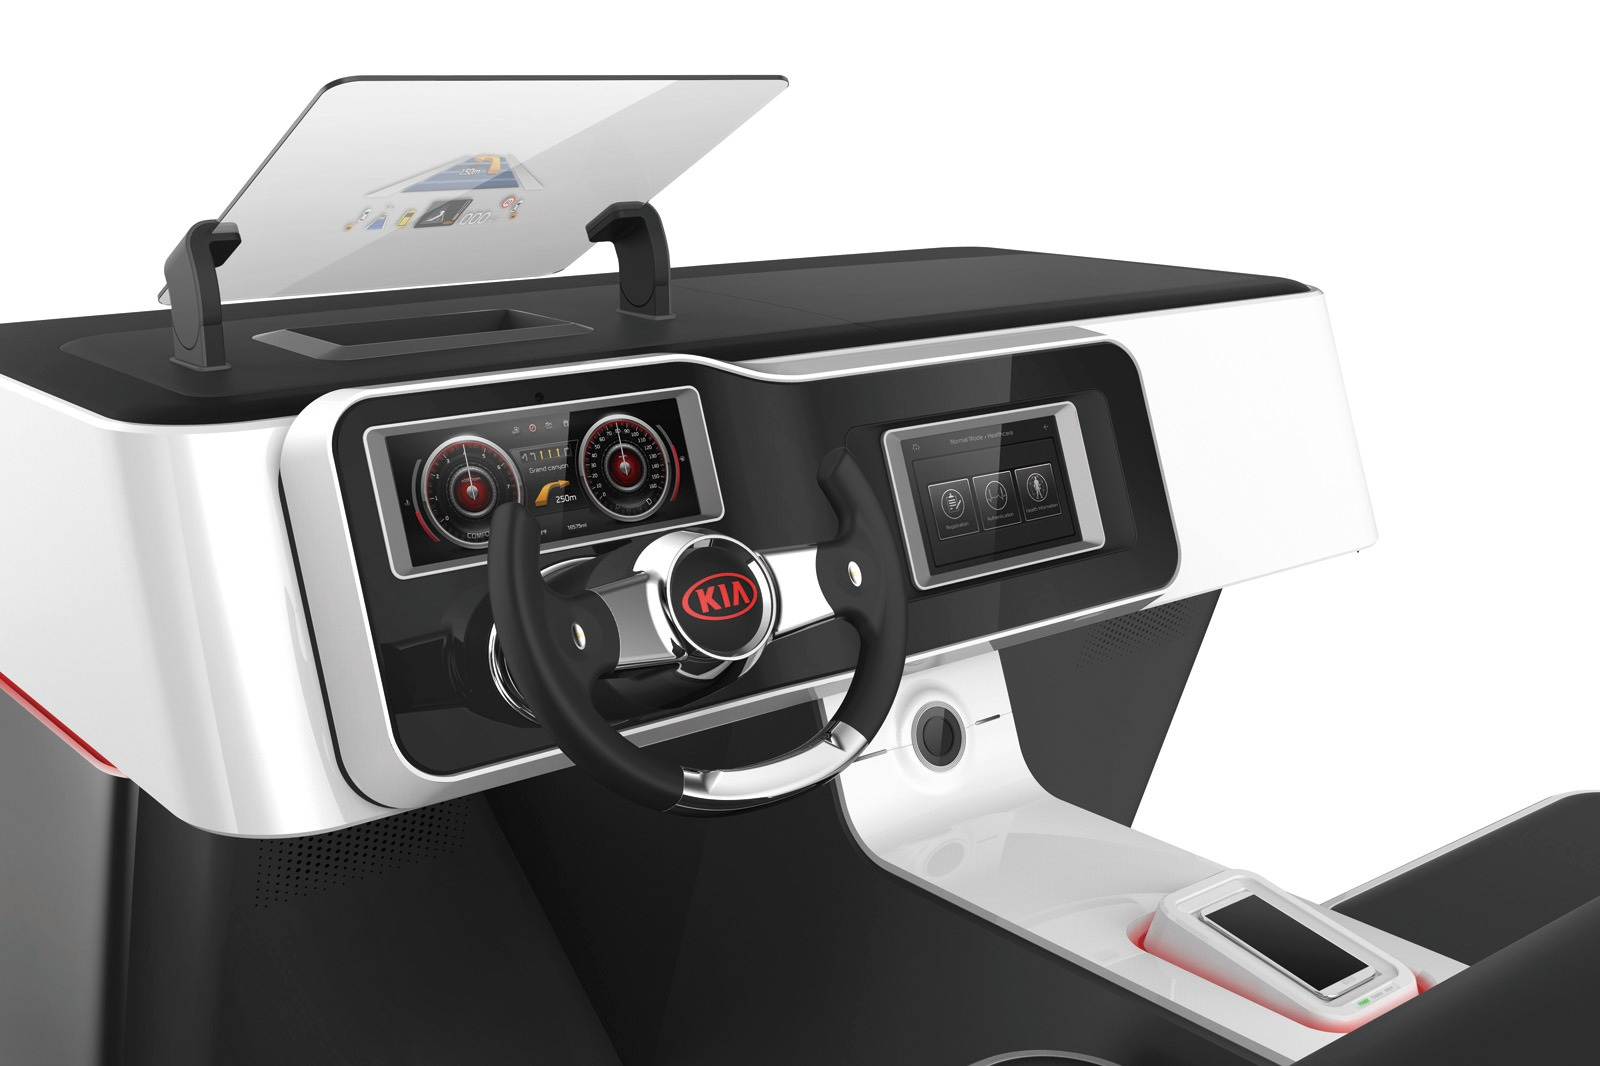
\includegraphics[width=4in]{images/kia.jpg}
\caption{Kia's UCD concept design}
\label{fig:kia}
\end{figure}

Although the Korean car-manufacturer have yet to specify when they will integrate their UCD concept into commercial vehicles but have promised consumers it will be released. 

Google have also entered the foray of In-Car Gestural Interaction with the recent acquisition of the motion control company Flutter \cite{flut}. Google aims to secure a patent for their unique idea of accepting free-motion gestures. Using multiple depth cameras that are mounted to the vehicle's headliner and a 3D laser sensor on the dashboard, Google's software engineers aim to create an approximation of the interior of the car. 
\begin{figure}[h!]
\centering
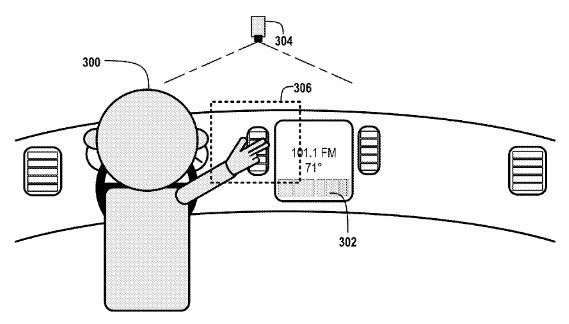
\includegraphics[width=4in]{images/google.jpg}
\caption{Google's gesture based car patent}
\label{fig:google}
\end{figure}

From this mapped interior, a dedicated CPU will determine the user's gesture, and the location that the gesture has been performed, to carry out an action, such as opening the window, or moving the driver's seat forward\cite{goog}.

These are just some of examples of the concepts car manufacturers have for gesture recognition - ford and Mercedes have also showcased some simple gesture designs at CES. Companies are investing a lot of time and resources to make freehand gesture controls a reality.

Although still mainly conceptual in nature, this the sheer number of concepts shows that some of the largest automotive manufacturers and software powerhouses in the industry are investing Research and Development into gestural interaction. Although these companies are strongly considering and showcasing gesture implementation, consensus is split. Most of these concepts are out with the scope of the research that will be conducted in this project but provide an interesting take on where the future lies. Just as touchscreens have permeated throughout society, so too will gesture controls in the coming years. The belief is that In-Car Gesture Interaction is the next desirable feature; the next evolution of input modality in the automotive industry.  

\section{Driver Safety}
\vspace{-3mm}
\subsection{Background}
\vspace{-3mm}
Driver distraction has long been recognized as one of the major contributors to roadside accidents (Treat et al., 1977). Drivers have always had the opportunity hamper their physical, visual and mental cognition through eating, communicating with the passengers in the car. They could also be on their mobile or be engaged in secondary activities that are unrelated to the current task of driving. However, over the years the potential for distraction has increased as in-vehicle technology has expanded. In the last decade, distracted driving came to the forefront of public awareness, stemming in large part from the rapid attachment rates and developments in mobile technology such as phones and the introduction of built-in peripherals and portable devices that are now widely available in vehicles. These devices allow drivers to engage in activities that were previously unimaginable (for example, setting a location on a GPS or connecting their phone to their car via bluetooth), and have the capacity to absorb drivers’ attention to a whole new degree. 

This concept of `Distracted driving' has received so much attention in recent years that it was designated the 2009 “Word of the Year” by Webster’s New World College Dictionary, becoming a safety-critical buzzword (U.S. DOT, 2010). To try and combat this, The U.S. Department of Transportation has held two summits with industry leading car manufacturers to discuss distracted driving and to identify opportunities for addressing the problem.

One of the primary concerns when implementing a new system within a car is the potential adverse effect it could have on driver safety. As found by National Highway Traffic Safety Administration (NHTSA), approximately 80\% of accidents occur due to a driver's negligence to concentrate on the road\cite{NHTSA}. This compiled with the fact that 65\% of rear-end accidents also occur because of the driver interacting with a system within their car highlights the safety concerns that exist within the industry.

The Royal Society for the Prevention of Accidents (RoSPA) also found that in 2012, of the 1,754 in car related fatalities, over 300 deaths can be attributed to driver distraction\cite{RoSPA}.  

The Virginia Tech Transportation Institute (VTTI) discovered\cite{VTTI} that drivers reaching to interact with an electronic device were 1.4 times more likely to be involved in a crash or near crash than non-distracted drivers. This is caused by the driver reaching for the control or looking at their center console when they should be attentive on the road ahead. 

In 2002, the NHTSA conducted a survey \cite{Royal} on approximately 4,000 licensed drivers to determine the potential distractions and interactions that drivers may face whilst on the road. Most respondents stated that on average drives, they were prone to talking to their passengers (81\%) and changing radio stations or looking for CDs (66\%). Half of the survey participants (49\%) reported consuming food or drink, while fewer reported using their mobile phone 
(25\%), Reading a map or directions while driving (12\%) and using telematics such as In-Car Navigation Systems(2\%).

As this survey was conducted in 2002, the wave of technological advancement had yet to occur and was nowhere near as prevalent as it is now. Built-in car navigation systems, that at the time of the survey's publication, were considered a luxury, are now viewed as a standardised add-on in modern vehicles and to many, a necessity. Mobile phones can be connected to a vehicle's central console via bluetooth or USB, giving the driver instant access to their contacts and music. Due to the proliferation of mobile phones and advancement of in-car technology, it can be assumed that since the time of the survey publication, these numbers have inflated significantly. These devices are much more commonplace and are more frequently used.

But how do you combat these erroneous mistakes that drivers make? Due to the emphasis and concern of  driver distraction, car manufacturers are now looking at how to mitigate this issue when implementing new technology. As previous findings have shown,\cite{345} gestural interaction can reduce the level of distraction that drivers face compared to haptic inputs, so if gestures as a form of input modality were globally accepted in vehicles, it has the potential to reduce the number of accidents caused through driver preoccupation. Of course, human error will still purvey, but {\it In-Car Gestural Interaction} offers a safer alternative than the current haptic input modality.

Based on the survey conducted by Royal \cite{Royal}, some distractions, such as focusing on passengers instead of the road and consuming food, can be attributed to common sense and driver awareness; human factors that are outwith a designer's control and are impossible to mitigate. However, {\it In-Car Gesture Interaction} can simplify many of the controls that are typically haptic-based. For example, changing to a different music artist whilst driving is visually, mentally, and cognitively demanding through a haptic modality. Gesture recognition within vehicles could remove such complexities and allow the driver to remain attentive visually to the road whilst interacting with the various systems in the car.   

Therefore the requirements of this project is to provide a safer alternative to controlling the various technology within vehicles and ultimately keeping the drivers cognition on the task of driving with the hope of reducing the risk of accidents.

\chapter{Requirements Gathering}
\label{sec:requirements}
\vspace{-3mm}
\section{Primary Requirements}
\vspace{-3mm}
\section{Functional Requirements}
\vspace{-3mm}

Provide a small sub-set of gestures that allow direct control of the main functions within a vehicle. 

Allow users to control the most desirable features in their car.

Provide a safer alternative to haptic controls through Gesture recognition, which could help mitigate accidents directly related to driver distraction.

Inform the user when they are detected by the device and in range top carry out tasks

Provide multimodal feedback based on an action. Audio feedback should be the primary form of feedback to allow the driver's focus to be maintained on reaching their destination safely. It is beneficial to also provide visual feedback for scenarios when the vehicles are stationary or if a passenger wishes to interact with the system.   

\section{Non-Functional Requirements}
\vspace{-3mm}
Ensure there is a latency or dwell time between gestures to prevent users from carrying out unwanted tasks.

Gestures should be simple and should not be time-consuming on the user. Therefore, multi-tiered gestures and cognitively demanding gestures will be prohibited. Gestures should take no longer than a second to complete, allowing their cognition to remain firmly on the road.

Gestures should not have a steep learning curve. They should be intuitive actions that are representative of the desired task. The Gesture device should also be responsive and reliable. If the user is unable to successfully perform gestures then the system will 

The area that gestures are recognise should be in a convenient 

\chapter{Design}
\label{sec:design}
\vspace{-3mm}
\section{Motivation}
\vspace{-3mm}
\section{Determining Device That Meets Requirements}
\vspace{-3mm}
Based upon the Functional and Non-Functional Requirements outlined in the previous chapter, it was discerned that only two commercial gestural recognition devices were suitable for the project. This section will outline the reasons for and against both the Microsoft Kinect and the LeapMotion and ultimately the device I have chosen to use.

\subsection{Microsoft Kinect}
\vspace{-3mm}
\subsubsection{Supporting Arguments}
\vspace{-3mm}
Due to the popularity of the Kinect, there has been a large adoption rate with developers that created gesture recognition software for the device. Microsoft's device is written in C\# and due to the significant development that has occurred with the LeapMotion, there is strong support online for the Kinect API. 

When the SDK was initially released, the gesture recognition was unreliable and limited. Through the number of developments that have occurred over the years, the gesture recognition libraries have improved substantially and the Kinect is now not only reliable hardware and software but also has a community of developers that are looking at ways to improve it further.
\begin{figure}[h!]
\centering
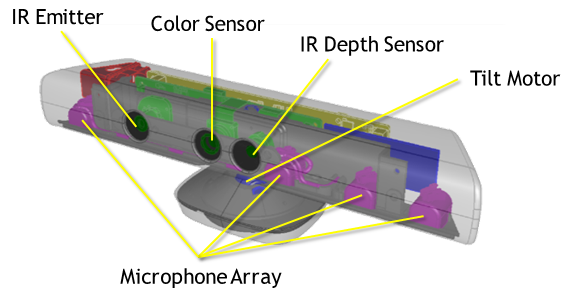
\includegraphics[width=4in]{images/KinectIR.png}
\caption{Kinect Hardware Components}
\label{fig:kinecthard}
\end{figure}

Furthermore, the Kinect is a robust piece of technology, capable of functioning as desired regardless of the light variance. This is due to the way in which the infrared emitter and depth sensor function, allowing the device to be capable of handling dramatic variances in light. In principle, the positional tracking is handled by its Infrared emitter, which transmits a factory calibrated pattern of dots across the spacial area and the Infrared depth sensor which reads the dot pattern. It can then determine the distance of objects in the defined space through a technique known as `time of flight', which works in similar principle to sonar, in that depending on how long the light is reflected back to the sensor determines its distance from the device. 

As vehicles can be driven at any period of the day and light often filters into the car and is amplified through the windows, it is important to be able to mitigate the changes to ensure that the hardware is always reliable to the end-user.
\begin{figure}[h!]
\centering
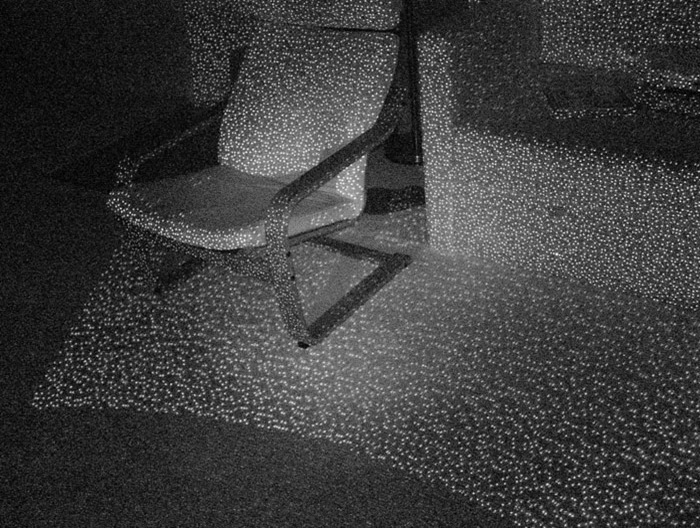
\includegraphics[width=4in]{images/irpattern.jpg}
\caption{IR Pattern Emitted Allowing Camera to Determine Depth}
\label{fig:irpattern}
\end{figure}

The Infrared is not the only functionality that is robust within the Kinect, as discovered by Anderson et al\cite{}. They found that the Kinect is also able to adapt to lens distortion, meaning that if the lens were to be slightly obscured or smeared, it would be able to compensate and the difference in its capturing would be negligible. 

This again is important as the interior of a car can experience fluctuations in temperature throughout the year and condensation may be a byproduct on the camera lens.

\subsubsection{Opposing Arguments}
\vspace{-3mm}
However, there are a number of reasons why Microsoft’s Kinect is not suitable for the project outline. With the first iteration of the Kinect, the device typically requires a full skeletal model of the person to operate efficiently, as defined by its API, to therefore accept any form of gestural input. Obviously, that is a major stumbling block for in-car gestural interaction as the driver will be sitting stationary and unless the Kinect could be angled in such a way to capture enough of their body, there is no assurance that their gestures will be approved by the device.

Furthermore, the skeletal tracking is limited in that it can only captures limbs and joints -- appendages such as fingers cannot be tracked effectively. This is a big issue for developing gestures within a car as the idea is to provide and promote a safer method of interacting with a car’s systems than the current haptic/ touch screen alternative. With the Kinect, the gestures would have to be profound and would feel obtuse within the confined area of the car. Let alone the fact that such large-scale gestures would potentially be more dangerous to the driver and be far more distracting and frustrating, especially if they  were not always approved as mentioned before.
\begin{figure}[h!]
\centering
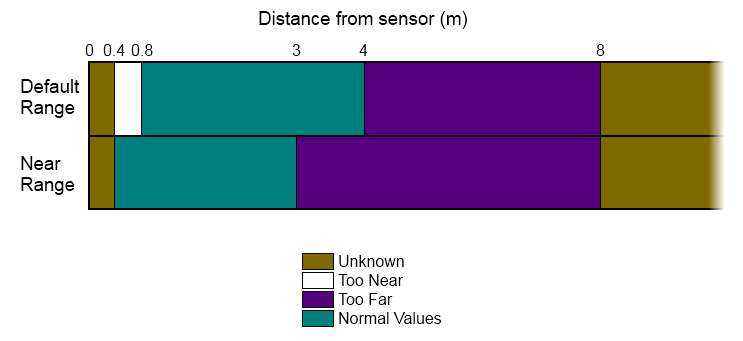
\includegraphics[width=4in]{images/KinectDistance.png}
\caption{Kinect's Field of View}
\label{fig:view}
\end{figure}

Finally and most importantly, the limitation of the Kinect’s depth resolution, frame-rate and depth space range really hamper its effectiveness within the car. Within the Kinect API, the DepthImageStream  Enumeration determines the resolution and frame rate of the depth stream. At maximum, the resolution of this depth can be 640x480 at 30 frames-per-second. This is why the Kinect is unable to detect small hand movements and gestures. Not only that but the Kinect requires quite a wide view before it will begin to recognise and accepts objects n its field. By default, objects must be at the very least 0.8 metres away before they can be interpreted by the Kinect – the infrared that is reflected back from any items or people closer than this range are discarded. Even with  Near Range mode enabled, the distance must still be 0.4 metres at minimum. The Kinect has a great range and field of view, up to 8 metres in Normal Range, but distance is not the desire, rather accuracy.

Microsoft recently released the Kinect II with the launch of their Xbox One which greatly optimises all of the issues I highlighted that would affect the objective of the project. However, as of this writing, they have they to announce any plans of releasing the device for PC or their API for development purposes.   

Taking these limitations into account and the confined, compact nature of a car’s interior, I did not believe that Microsoft’s Kinect was a viable gestural input device for this particular project. Especially as safety is the primary concern for the driver and from the offset, granted without any development, it seems like the Kinect would be a further distraction rather than a deterrent. The aim is to have the gestures as small-scale as possible and they should not detract from the objective of driving. With the Kinect, that simply would not be feasible.
\subsection{LeapMotion}
\vspace{-3mm}
\subsubsection{Arguments For}
\vspace{-3mm}
As the LeapMotion is specifically designed to track hand movements that is unequalled by any other gestural device, it has a huge advantage in the field for recognising small deviations accurately.   
The smaller observation area and higher resolution of the device differentiates the product from the Kinect, which is more suitable for whole-body tracking in a space the size of a living room.
\subsubsection{Arguments Against}
\vspace{-3mm}
At the time of this project, the released version of the LeapMotion SDK is incapable of skeletal tracking, which presents issues as the device is in unable to differentiate between fingers -- it can only determine how many fingers are ``visible''. Finger visibility presents another issue as the device captures a significant number of frames per second, it picks up a lot of erroneous noise from a hand, such as a finger that is closed. This problem seems to vary from person to person; for some, even when clenching their fist tightly, the LeapMotion may recognise a knuckle as an appendage. 

\section{Gesture Elicitation}
\vspace{-3mm}
With the objects that the users will interact with in the car defined, the next step in the process was to determine what gestures would be suitable for not only each interaction, but also for the confined space within the car. Classification of gestures has been explored in previous academic research papers but not specifically for in-car interaction. Google’s innovative patent conceptually looks at interacting with the cars systems via locality (gesturing your hand down when near a window opens the window, gesturing near air-conditioning turns it on etc.) but given the LeapMotion’s limited range and infra-red sensitivity, following such a prototype is not applicable.

To find out what gestures were intuitive to users, a gesture elicitation experiment was carried out to determine if the gestures can be standardised. It is important to conclude which gestures feel familiar and intuitive to each action before developing the interactions themselves. One person’s interpretation could be vastly different to the majority so it is vital to obtain a cross-section of participants from varying backgrounds and age.

\begin{figure}[h!]
\centering
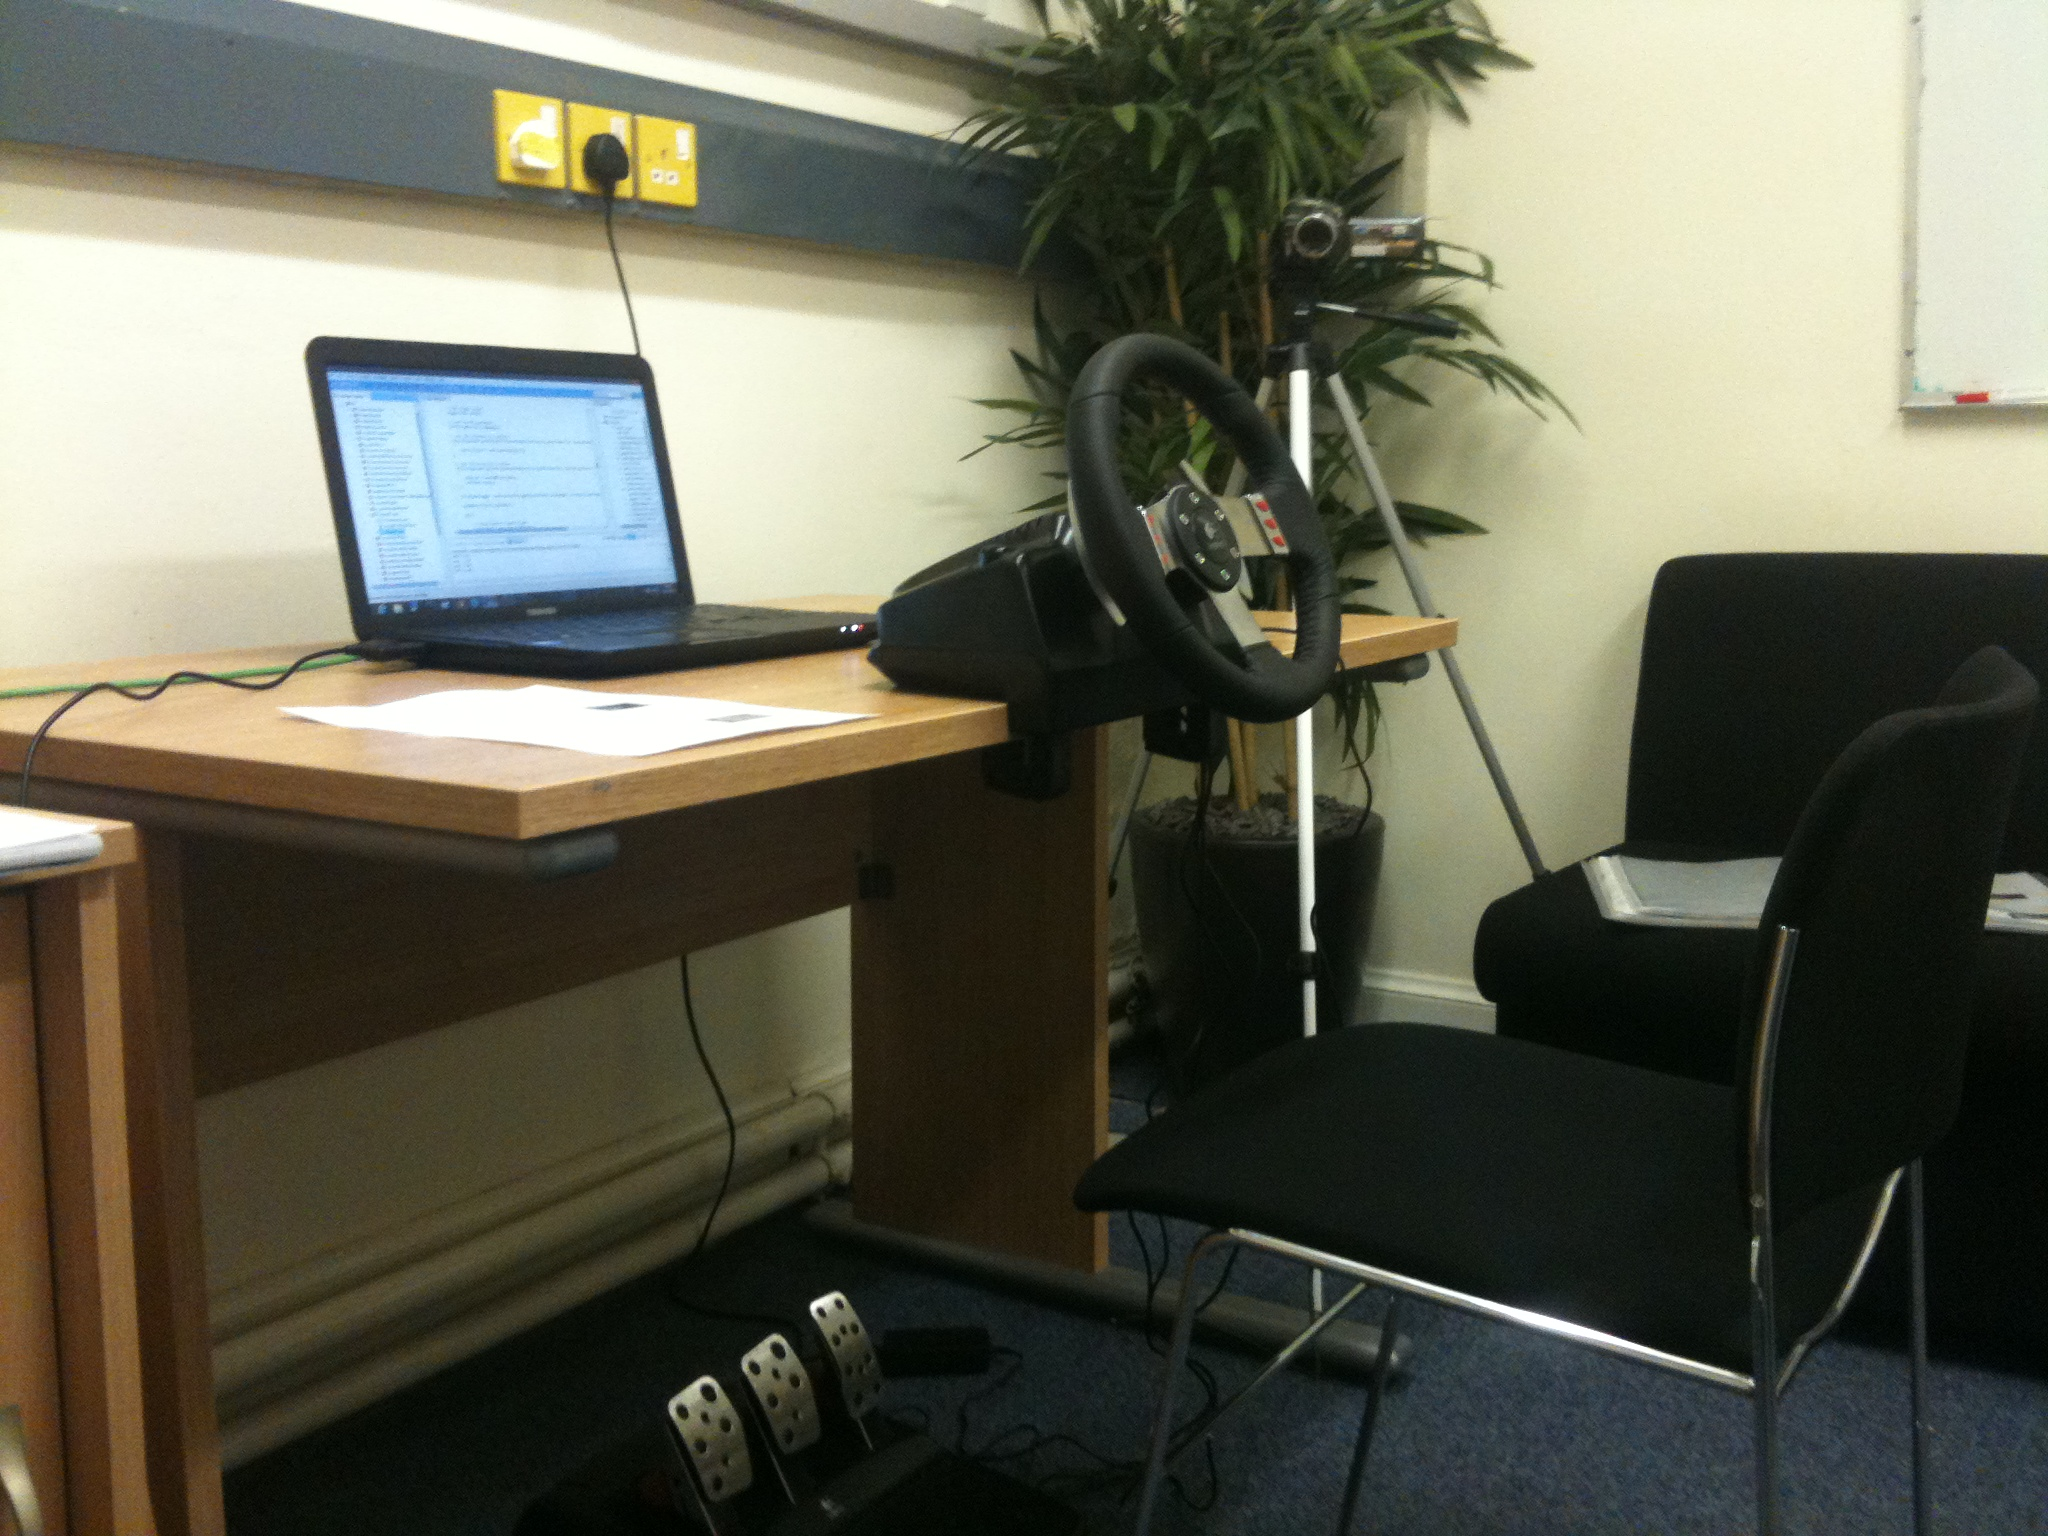
\includegraphics[width=4in]{images/Requirements.jpg}
\caption{Usability Lab Configuration}
\label{fig:sawb}
\end{figure}

In order to do this, 13 participants (12 men and 1 woman) took place in the experiment were they were ask to carry out a series of tasks, using the gesture that they felt was natural to each scenario. This allowed not only relations to be found between interactions, but also to classify the types of gestures.

The experiment was carried out in the Usability Lab of the Sir Allan Williams building. Participants were asked to carry out certain gestures whilst focusing on their road awareness in a driving simulator. This driving simulator was provided via OpenDS (insert website at bottom of page).

Using a think aloud approach, users were also encouraged to speak openly regarding their tasks and their overall opinion of interacting with an automobile’s systems whilst driving as they took part in the experiment.

With the appropriate ethics approval and knowledge that they could end the experiment at any point if they felt uncomfortable (See Appendix), participants were filmed so that the requirements elicitation could be analysed and documented.

\subsection{Classification of Gestures}
The gestures that participants could use fell into two categories:

\begin{easylist}[itemize]
& \textbf{Small-Scale gestures}, in which either both their hands stay on the wheel or one hand slightly off the wheel. These can be further categorised as:
&& \textbf{Finger gestures} -- rotating a finger, pointing gestures and counting the number of fingers shown by participant.
&& \textbf{Hand gestures} -- swiping and open/closed hand gestures.
& \textbf{Free-Motion gestures}, which could be a motion towards their head, two handed gestures or a variety of miscellaneous movements. These can also be further classified as:
&& \textbf{Mimic gestures} -- Hand gesture towards ear, body part or object within the vehicle.
&& \textbf{Grandiose gestures} -- Two hand gestures or head and body movements.
\end{easylist}

Users were asked to attempt to primarily use small-scale gestures and if they could not think of a suitable movement to represent the action, then they should opt for a free-motion gesture.  For the majority of scenarios, relations existed between the gestures that users felt best represented the action.  It is important to note that participants were not informed of the hardware limitations that exist with the LeapMotion – the purpose was to find the common, natural gestures for each interaction. This experiment was technology agnostic; finding acceptable gestures was the sole purpose on which software developers could adhere to. As technology progresses and gesture technology becomes more widespread and relevant (the addition of depth cameras and improved tracking technology), the findings of the experiment could be beneficial to off-device interface designers and others aiming for free-motion gesture recognition techniques 

The following sections will document each category of the gesture elicitation process and the requisite findings.

\subsection{Main Menu}
\vspace{-3mm}
Within modern vehicles, a built-in central console allows the driver to navigate to music, GPS, their phonebook and other periphery systems within the car. Naturally, the first step in the requirements elicitation was to determine the gestures the participants would use to navigate such a menu. Participants were provided with a visual representation of a typical menu within a car’s central dock.

Four scenarios were presented in controlling a menu and whilst continuity existed between participants for the first three actions, the forth scenario contained a variety of different gestures.

Participants were informed that the gestures they selected for menu interaction would apply throughout the rest of the experiment.

\subsubsection{Navigating Through the Menu}
\vspace{-3mm}
As gestures are becoming prevalent throughout society, given the worldwide appeal and acceptance of gestural touch screens, people intrinsically know how to interact and navigate with touch and gesture-based interfaces. These are common pre-defined gestures, regardless of the developer or mobile operating system. This was highlighted in the requirements elicitation for navigating as the majority of the participants selected a gesture that is commonplace within mobile devices.

\begin{figure}[h!]
\centering
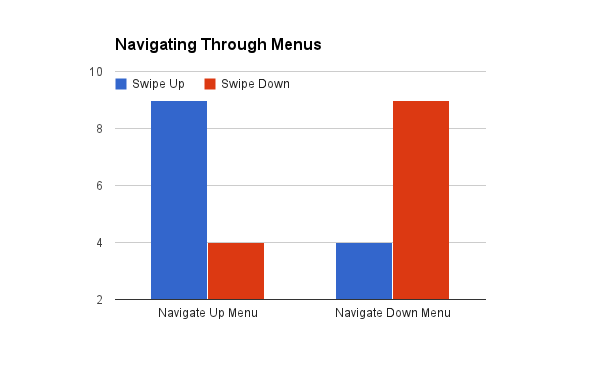
\includegraphics[width=6in]{images/Navigate_Menu.png}
\caption{Menu Navigation Results}
\label{fig:sawb}
\end{figure}
\newpage

Nine participants swiped in the direction requested whereas a few inverted the gestures, swiping down to go up the menu and the opposite for going up the menu. The reasoning the minority chose to invert the swipe gesture is most likely due their familiarity with mobile phone interface gesture recognition patterns – most touch devices invert the motion for swipe movements, making a swipe up on the screen scroll down and vice versa. One participant explicitly discussed their thought process when determining which gesture they would use for navigation:

\begin{table*}[!ht]
\hfill{}
\texttt{
\begin{tabular}{@{}p{-50mm}p{25mm}p{120mm}@{}}
& \textbf{Participant:} & "I guess it depends...if I was using my phone, I would swipe down to scroll up. But if I was using my pc, I would gesture down to the next option." \\\\
& \textbf{Myself:} & "The important aspect to remember is that you are not directly interacting with a physical object. The gestures you are doing are in the ether."  \\\\
& \textbf{Participant:} & "Yeah. Will there be enough options in a menu for the velocity of the gesture to matter? Like if I swipe my hand quickly will it scroll through the menu faster?" \\\\
& \textbf{Myself:} & "As this is a proof of concept, it will only have four options – Music, GPS, Contacts and Extra features" \\\\
& \textbf{Participant:} & "In that case I would emulate what I do on my phone and invert the direction – down to go up and up to go down"\\
\end{tabular}
\hfill{}
}
\caption{Conversation Regarding Gesture Familiarity}  \end{table*}

\subsubsection{Selecting an Option}
\vspace{-3mm}
All participants found that a gesture symbolic of a  "screen tap" was the best method to select an option from the menu. Again, this is due to gesture familiarisation with other touch interfaces as it is certainly a clear and evident way to choose one item from a list of options.

It is worth noting that several participants specified that they would swipe to the menu option they desired until it was highlighted and then select it. This was preferred over having than the options existing in a virtual space; the screen-tap gesture should not rely on accuracy or locality in space -- especially whilst the car is in motion -- but only on the hand recognition.

\subsubsection{Revert to Previous Menu}
\vspace{-3mm}
The last menu-related task produced a variation of actions from participants, unlike the previous choices. In fact, the participants were evenly split as \cite{} shows. Although the gestures were ostensibly different, they are similar in nature, only in axis of space.

\begin{figure}[h!]
\centering
\begin{subfigure}[b]{0.4\textwidth}
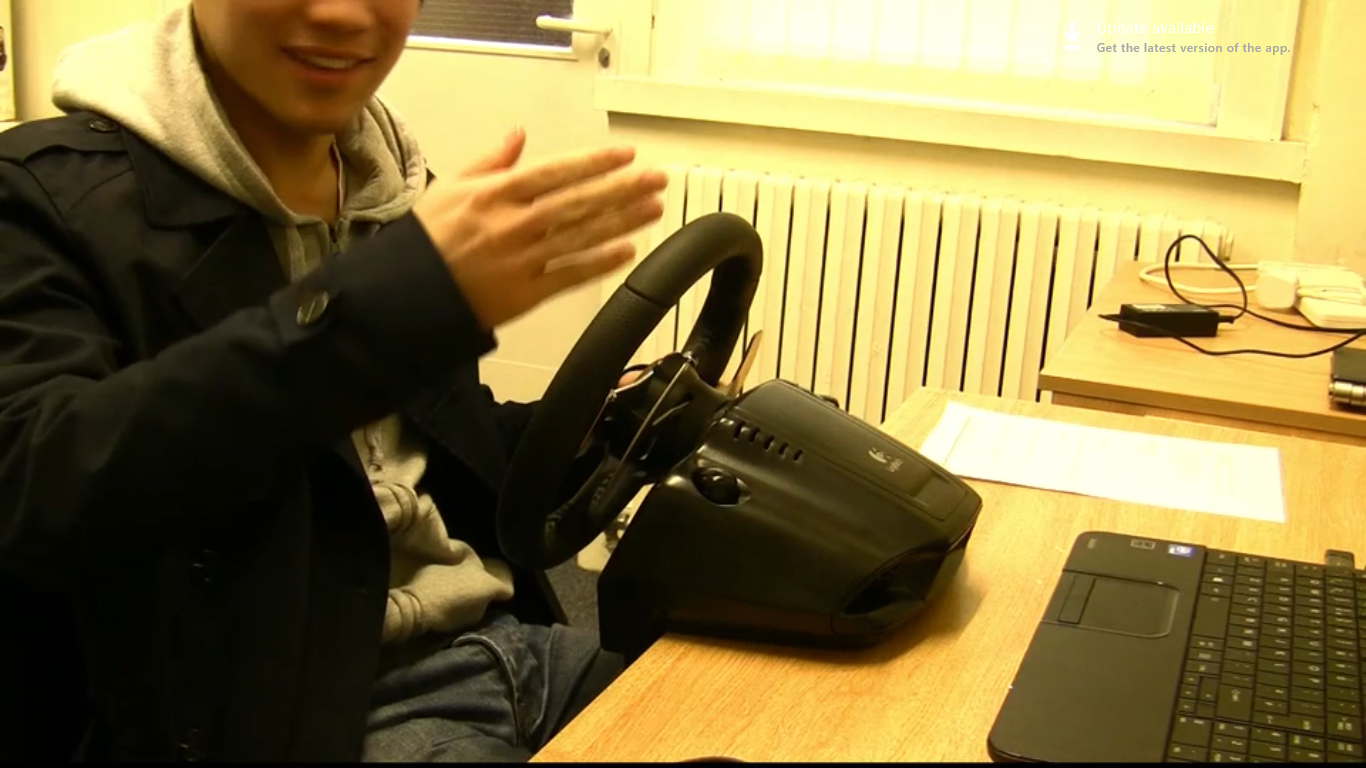
\includegraphics[width=\textwidth]{images/SwipeLeft.png}
\caption{Swipe Left}
\label{fig:swipeleft}
\end{subfigure}
~ %add desired spacing between images, e. g. ~, \quad, \qquad etc.
%(or a blank line to force the subfigure onto a new line)
\begin{subfigure}[b]{0.4\textwidth}
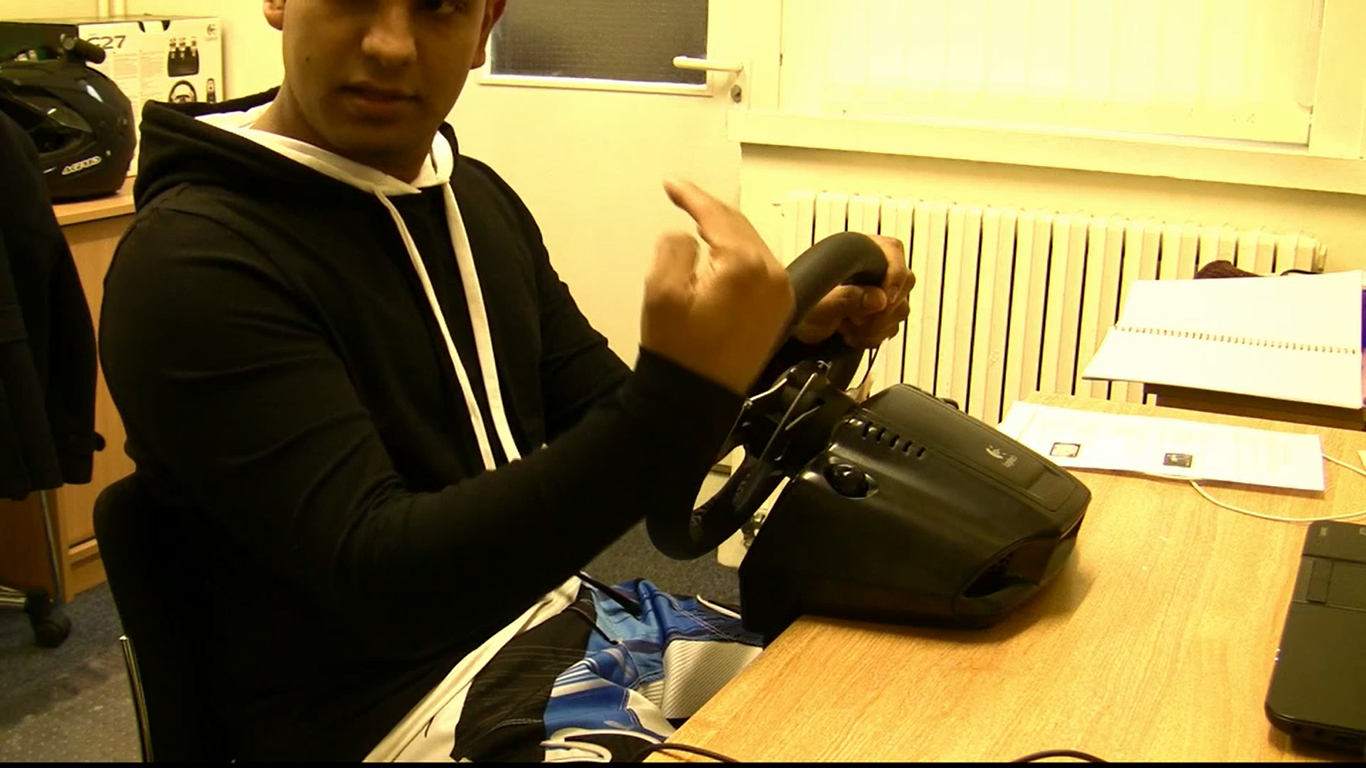
\includegraphics[width=\textwidth]{images/beckon.png}
\caption{Beckon towards body}
\label{fig:beckon}
\end{subfigure}
~ %add desired spacing between images, e. g. ~, \quad, \qquad etc.
%(or a blank line to force the subfigure onto a new line)
\caption{Gestures for Returning to a Previous Menu}\label{fig:goback}
\end{figure}

54\% of the participants felt that swiping to the left was the best way to return to an option, due again to their pre-existing gesture familiarity, whilst 38\% preferred gesturing their hand towards their own body, resembling a “come to me” gesture. Without a clear preference, I would suggest using a gesture that will be unique throughout. This will be explored in further detail in the next sections.

\subsubsection{Suggested Gestures}
\vspace{-3mm}
Given the participants overall agreement and familiarity with these gestures, I would suggest the following gestures for each interaction. Despite the relatively low number of participants, I believe that the same results would appear with a larger demographic. Even if the users did not-have any pre-existing recognition with gesture technology, they would be able to adapt and recognise the natural motions of the gestures selected and what they represent in each case.

\begin{table}[h!]
\centering
    \begin{tabular}{|l|l|l|}
    \hline{}
    \textbf{Task}                    & \textbf{Gesture}      & \textbf{Classification} \\ \hline
    Scroll Up               & Swipe Up     & Hand Gesture   \\ \hline
    Scroll Down             & Swipe Down   & Hand Gesture   \\ \hline
    Select an Option        & "Screen Tap" & Hand Gesture   \\ \hline
    Return to Previous Menu & "Beckon"     & Hand Gesture   \\ \hline
    \end{tabular}
\end{table}

For gesturing to go back to a previous menu, although the majority of participants suggested swiping left to return to the previous set of choices, this may result in gesture confusion which will be further explored in section blah blah, as the gesture is also suited to another scenario. Therefore I would recommend a unique gesture that will not create driver confusion and frustration with the gesture input mechanism. Ultimately, such problems could lead to their attention being removed from driving, which is the adverse aim of the project. 

determine which of the two designed gestures users adapt to more naturally and can be detected by the LeapMotion.
\subsubsection{Gestures Defined for \textbf{\textit{In-Car Gestural Interaction}}}
\vspace{-3mm}
Given the simplicity of the gestures used by participants and most of the gestures are predominately associated with said tasks, I have decided to use the same gesture for all but one, navigating back to a previous menu. 

This is to avoid gesture conflict that may occur when zooming in and out a map, which will be discussed in section blah blah, I felt it was best to use a unique gesture for the action. As the LeapMotion in theory can differentiate gestures based on the number of fingers in a swipe, I decided to use a two finger swipe left movement to signify returning to previous set of options. Although this will have a slight learning curve for users, this seems to be the most sensible option in order to ensure that gesture conflict does not occur resulting in the user making an undesired choice.
\begin{figure}[h!]
\centering
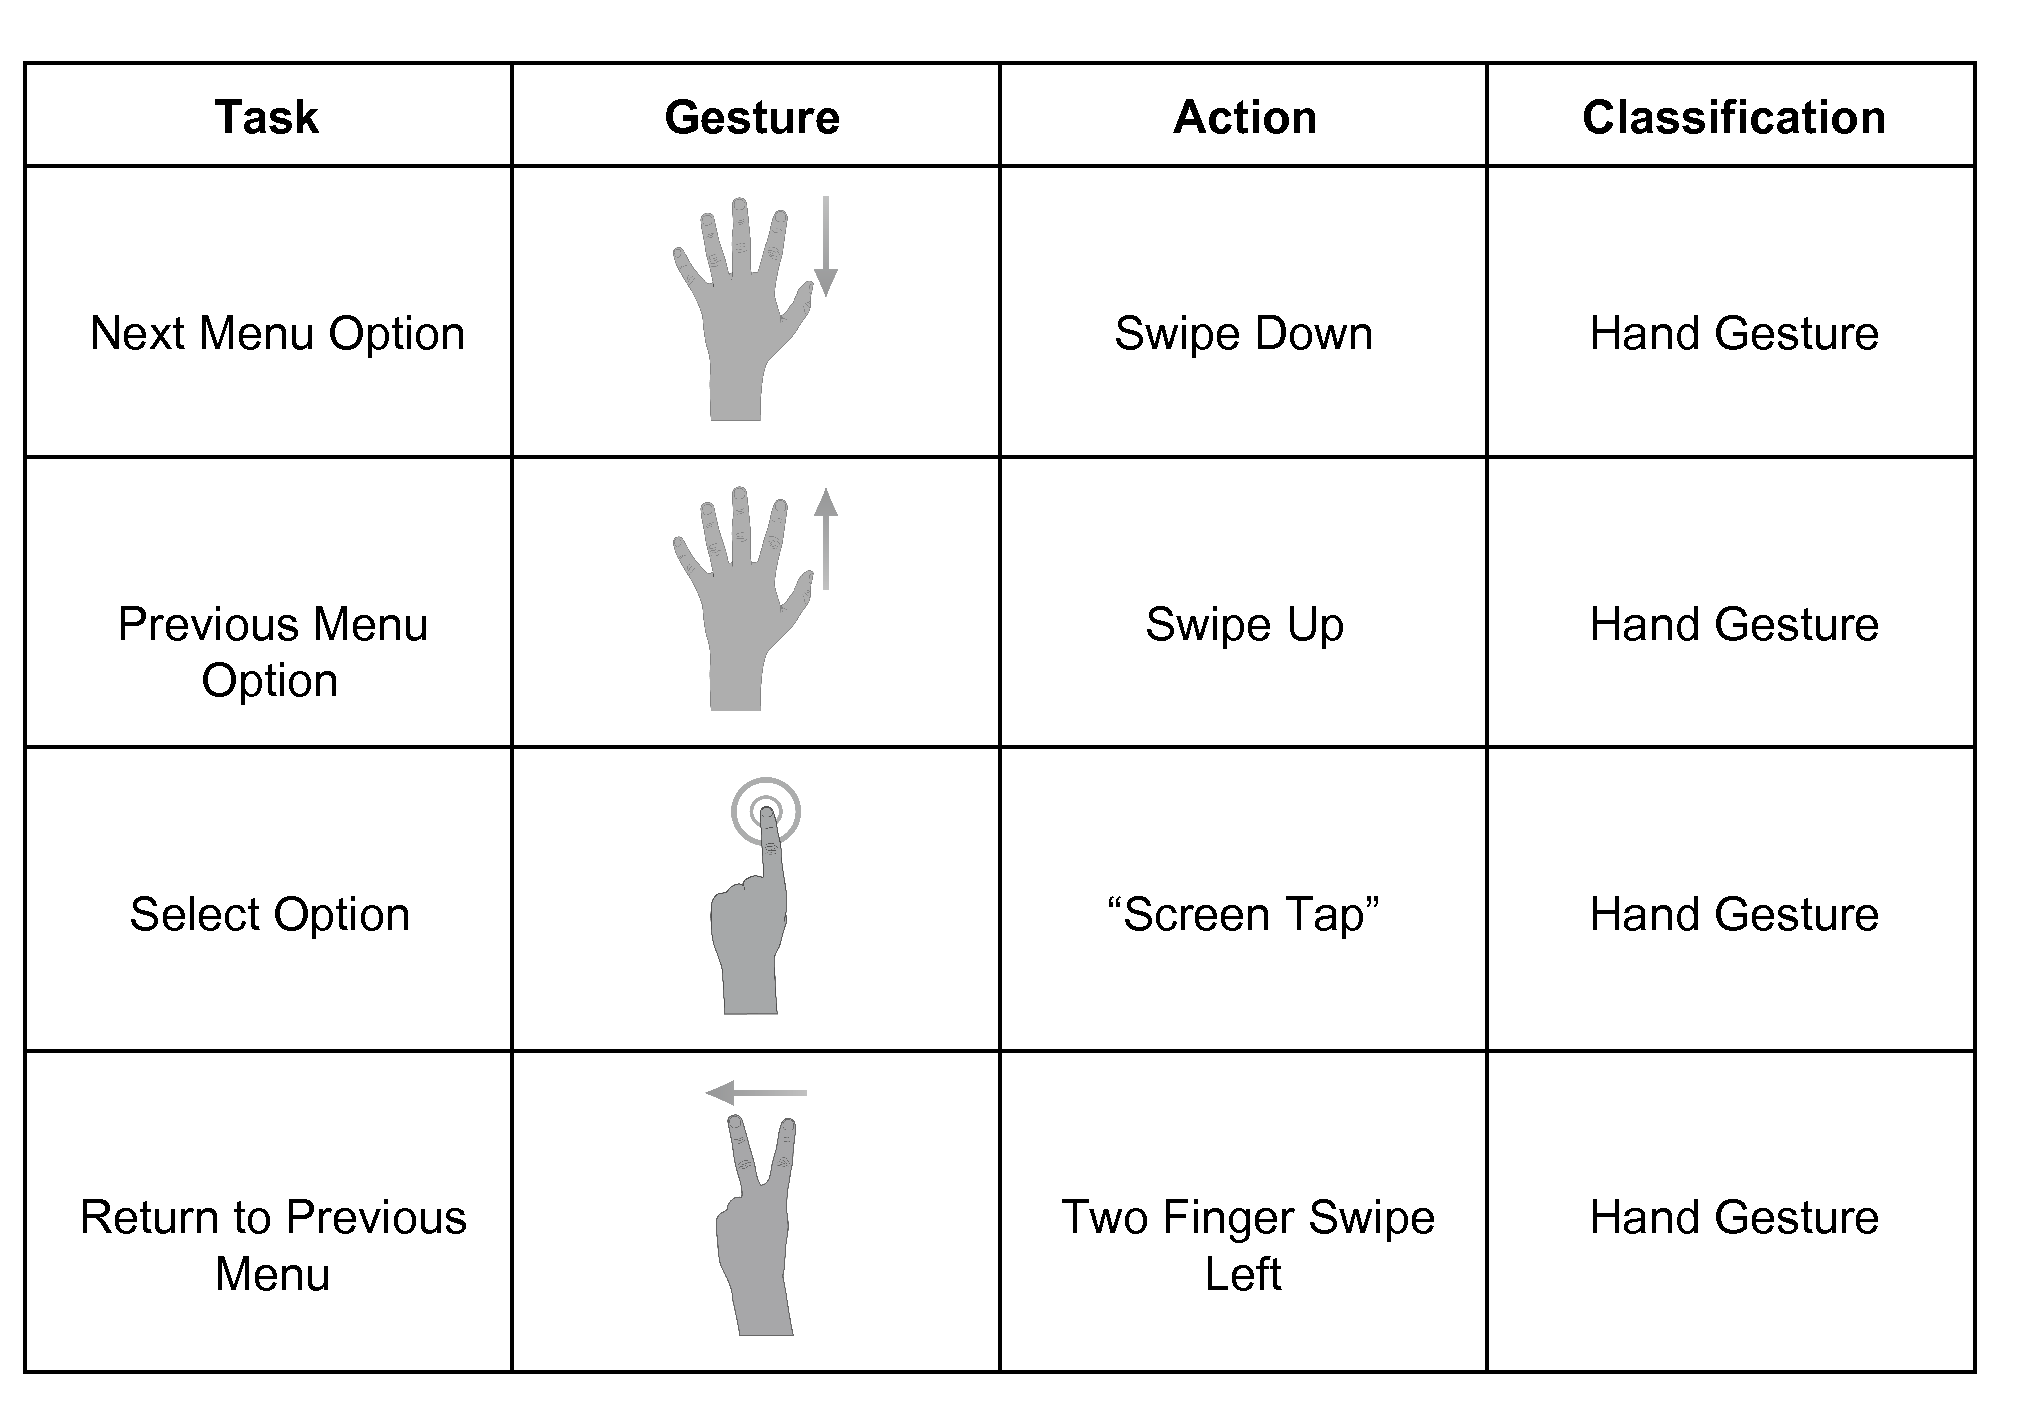
\includegraphics[width=6in]{images/LeapMenuGesture.png}
\label{fig:leapmenu}
\end{figure}
\newpage

\subsection{Music}
\vspace{-3mm}
Within modern car stereo systems one can expect Bluetooth functionality, allowing the driver or passenger to sync their music device to the vehicles built-in console. Although this is now common practice, the way the user then controls their music is often awkward as they have to use the controls from the central console. More importantly, this could be potentially hazardous whilst driving as it requires visual and mental cognition. Although some of the music features can be controlled through haptic controls on the steering wheel, an off-device gesture alternative is worth exploring.

Considering the NHTSA's survey on this matter\cite{Royal}, it is especially important to determine if a series of small-scale gestures can be used to reduce the intensity on as driver's overall cognition. 

As the gestures used for interacting with menus apply when choosing artists and songs, only music-specific gestures were tested. 

\subsubsection{Play/Pause}
\vspace{-3mm}
Consensus was strong amongst the participants that playing and pausing the current song should use the same gesture as selecting an option, in the same way that they would press play on their music device.

\subsubsection{Increasing and Decreasing Volume}
\vspace{-3mm}

For altering the volume, opinion was divided somewhat as the best from of interaction. 

As figure blah blah shows 69\% of the participants felt that rotating clockwise and anti-clockwise to increase and decrease the volume respectively was the best approach to alter the volume. This can be attributed to their familiarity with rotational knobs for volume control and audio devices such as iPods, where rotations signify a change in volume when a song is currently playing.

The other 31\% of participants felt that gesturing up and down were preferable, suggesting a rise and fall of volume. Both options are entirely valid.

\subsubsection{Next and Previous Song}
\vspace{-3mm}

Skipping to the next and previous songs was a simple task for the participants. Every person that took place in the experiment carried out the same gestures -- A swipe left to go to the previous song and a swipe right to the next song

This was primarily due to familiarity with audio controls – to skip to the next song, the respective skip next button is always to the right, adjacent to the play/pause. Similarly, the haptic button for the previous song is always on the opposite side. As such, the choice for the participants was therefore an instantaneous reaction.

\subsubsection{Suggested Gestures}
\vspace{-3mm}

Given how natural the gestures used throughout the music options were to users, I would suggest the following irrespective of technical limitations:

\begin{table}[h!]
\centering
    \begin{tabular}{|l|l|l|}
    \hline
    Task            & Gesture               & Classification \\ \hline
    Play            & "Screen Tap"          & Finger Gesture \\ \hline
    Pause           & "Screen Tap"          & Finger Gesture \\ \hline
    Next Song       & Swipe Right           & Hand Gesture   \\ \hline
    Previous Song   & Swipe Left            & Hand Gesture   \\ \hline
    Increase Volume & Rotate Clockwise      & Finger Gesture \\ \hline
    Decrease Volume & Rotate Anti-Clockwise & Finger Gesture \\ \hline
    \end{tabular}
\end{table}

Not only are these gestures familiar to users, they are also simple in execution and should hopefully provide a better alternative to haptic controls.

\subsubsection{Gestures Defined for \it{In-Car Gestural Interaction}}
For this project, all of the preferred gestures suggested by the participants are viable as they can not only be detected by the LeapMotion, but should also be simple to execute. Therefore the suggested gestures will be replicated in implementation.
\begin{figure}[h!]
\centering
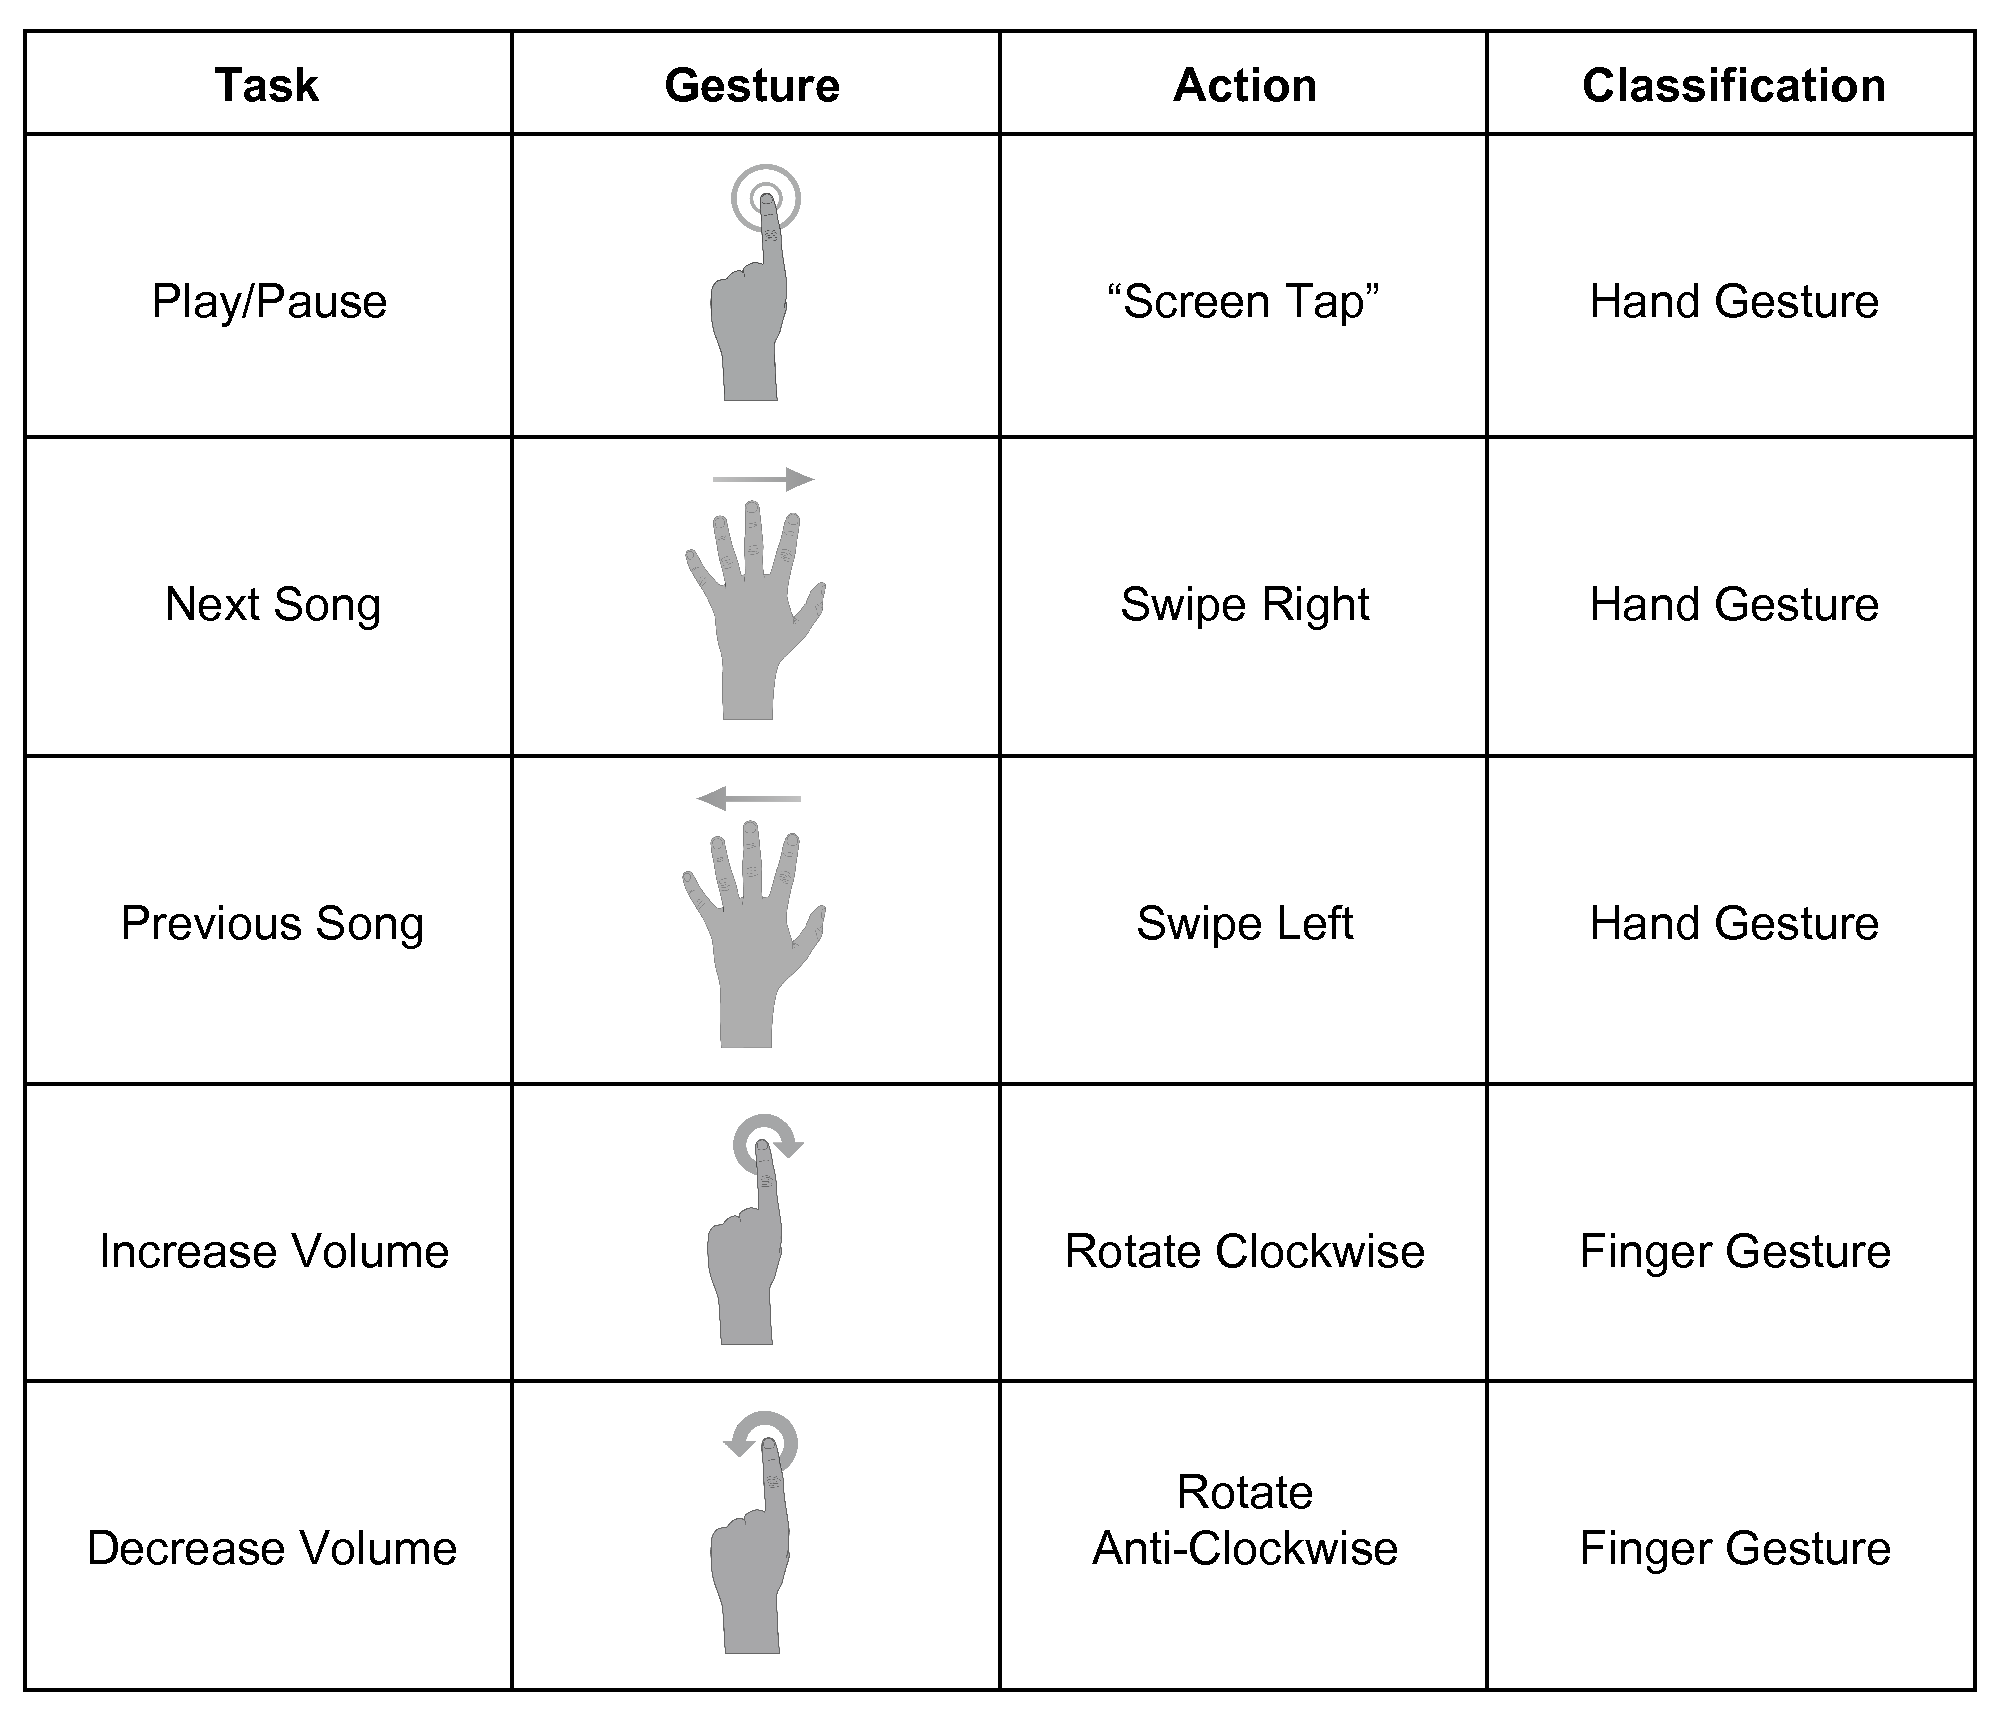
\includegraphics[width=6in]{images/LeapMusicGestures.png}
\label{fig:leapmusic}
\end{figure}
\newpage

\vspace{-3mm}
\subsection{GPS}
\vspace{-3mm}
With the adoption of Navigation Systems within the automotive industry, it is now commonplace to find a GPS built into a car's central console dock. People are no longer confined to analog, physical maps, meaning that the physical layer of cognition has been removed as a result. However, GPS systems have spawned a plethora of new safety concerns.

Although drivers should solely follow plotted directions and remain attentive to their surroundings whilst driving, it is likely that they will enter directions on the move and attempt to observe their surrounding area with the software. This will mainly be controlled by either a touch screen or through built-in controls, which could result in potentially hazardous scenarios.

The following sections will observe the gesture alternatives that participants felt resembled the actions found in a common GPS.

It is worth noting that when searching for a location or seeking directions, drivers are strongly advised to do so whilst stationary. In reality, it is unlikely that all drivers will adhere to such practices. This project does not condone such behaviour.

\subsubsection{Zoom In and Zoom Out}
\vspace{-3mm}
The participants were divided into two categories of gestures for the best way to zoom in and out of a map.

Pinching gestures have become standard in mobile applications and it is an action that is now used intuitively for zooming in and out. Given this, 10 or the 13 participants instantaneously used pinching in and out to control zooming. 

The remaining three participants felt that pushing in and out was more synonymous with controlling zoom. As they were not constricted to touching a device, they considered these gestures to be preferable given the freedom of their movement.

\subsubsection{Place Marker}
\vspace{-3mm}
All users determined that a `screen tap' gesture was sufficient for placing a marker on the map. Accuracy would be a slight concern if the locality hand position is not tracked but given that the purpose of this gesture elicitation is to find the best methodology, this is not a primary concern.

\subsubsection{Scrolling}
\vspace{-3mm}
In a similar fashion to the zooming methods in section blah blah 10 users implemented hold and move gestures which the remaining three users opted for swiping in the desired direction. Interestingly,  the users were divided in the exact same way, signifying a difference in gestural ideologies.

The majority chose this tactic due to mobile standardisation once again. Their idea was that whilst their hand was in a forward state, a movement in any direction will be represented on the map. 

\subsubsection{Suggested Gestures}
\vspace{-3mm}
\begin{table}[h!]
\centering
    \begin{tabular}{|l|l|l|}
    \hline
    Task            & Gesture               & Classification \\ \hline
    Zoom In            & `Pinch In'          & Hand Gesture \\ \hline
    Zoom Out           & `Pinch Out'          & Hand Gesture \\ \hline
    Scroll       & Hold and Move           & Hand Gesture   \\ \hline
    Place Marker   & `Screen Tap'            & Finger Gesture   \\ \hline
    \end{tabular}
\end{table}

\subsubsection{Gestures Defined for \textbf{\textit{In-Car Gestural Interaction}}}

\subsection{Contacts}
\vspace{-3mm}
With the progression of mobile technology, the potential for drivers to use their phone for calls has become a genuine concern for road safety and distraction prevention.

Taking into consideration users ability to connect their phone to their car through axillary cables, bluetooth and new concepts such as Apple's CarPlay\cite{}, most modern cars have microphones to pick up the driver's voice to allow them to communicate. However, the problem still exists that they have to physically interact with either their phone or the central console, which can be cognitively demanding in certain situations (imagine a scenario where a person needs to answer an urgent call and deviates their focus as a result).

As the mitigation of accidents is the one of the primary non-functional requirements for this project, it is of importance to determine if gestural modality for phone interaction is beneficial to safety.

This section will evaluate the core controls that a driver should have at their disposal. As with previous menus, the gestures for navigating between options will apply for moving between contacts.

\subsubsection{Call Contact}
\vspace{-3mm}
Given the high frequency of phone usage worldwide, mobile phones have become an integral part of society, to the point that it would now be uncommon for someone not to have their mobile always at their disposal. The ``call me'' hand gesture is perhaps the most iconic interpersonal gesture that occurs in daily life, regardless of location or culture.

Given this ease of recognition, all of the participants reacted, almost in unison, by emulating picking up a phone to communicate.  One participant even stated, ``Would anyone use any other gesture?''

\subsubsection{End Phonecall and Reject Incoming Call}
\vspace{-3mm}
In a similar fashion, all of the participants decided to hang up their imaginary phone, gesturing down towards the steering wheel. 

\subsubsection{Suggested Gestures}
\vspace{-3mm}
The uniformity of gestures chosen for the Contact menu presents an interesting topic -- gestures relating to communication appear to be agnostic of age and are hence relevant to different generations of potential end-users. Although this experiment was only carried out to a small subset of people, one could believe that this trend would continue.

\begin{table}[h!]
\centering
    \begin{tabular}{|l|l|l|}
    \hline
    \textbf{Task}             & \textbf{Gesture}         & \textbf{Classification} \\ \hline
    Call Contact     & "Pick Up Phone" & Mimic Gesture  \\ \hline
    End Conversation & "Hang Up Phone" & Mimic Gesture  \\ \hline
    Reject Call      & "Hang Up Phone" & Mimic Gesture  \\ \hline
    \end{tabular}
\end{table}

Therefore, I would highly recommend implementing these gestures in any application that has designated gesture controls relating to communication or conversing. 

\subsubsection{Gestures Defined for \textbf{\textit{In-Car Gestural Interaction}}}
\vspace{-3mm}
\begin{figure}[h!]
\centering
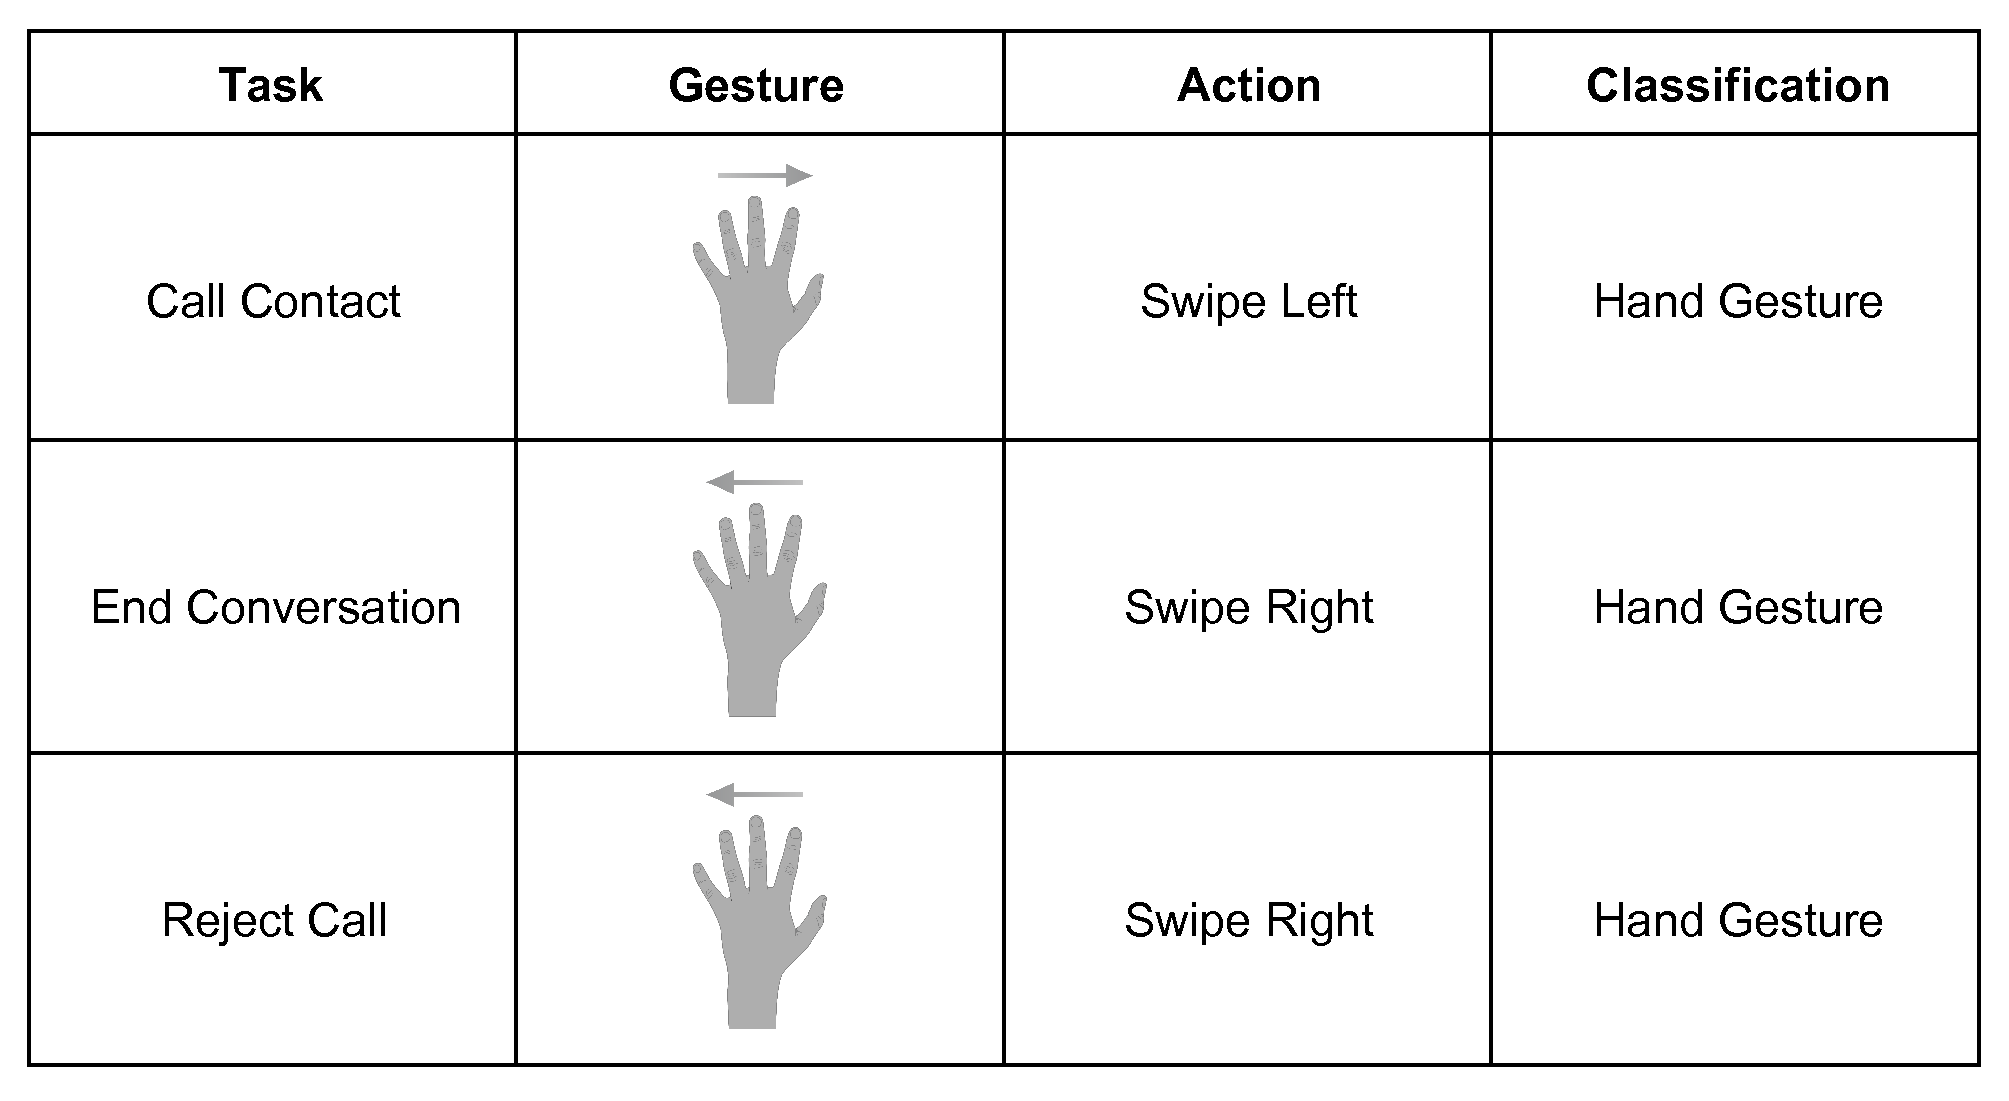
\includegraphics[width=6in]{images/LeapContactGestures.png}
\label{fig:leapcontacts}
\end{figure}

\subsection{Air-Conditioning}
\vspace{-3mm}
\subsubsection{Increasing and Decreasing Fan Strength}
\vspace{-3mm}
\subsubsection{Increasing and Decreasing Temperature}
\vspace{-3mm}
\subsubsection{Suggested Gestures}
\vspace{-3mm}
\subsubsection{Gestures Defined for \it{In-Car Gestural Interaction}}
\vspace{-3mm}
\subsection{Windows}
\vspace{-3mm}
\subsubsection{Opening and Closing the Driver-side Window}
\vspace{-3mm}
\subsubsection{Opening and Closing the Passenger-side Window}
\vspace{-3mm}
\subsubsection{Opening and Closing the Both Windows Simultaneously}
\vspace{-3mm}
\subsubsection{Suggested Gestures}
\vspace{-3mm}
\subsubsection{Gestures Defined for \it{In-Car Gestural Interaction}}
\begin{figure}[h!]
\centering
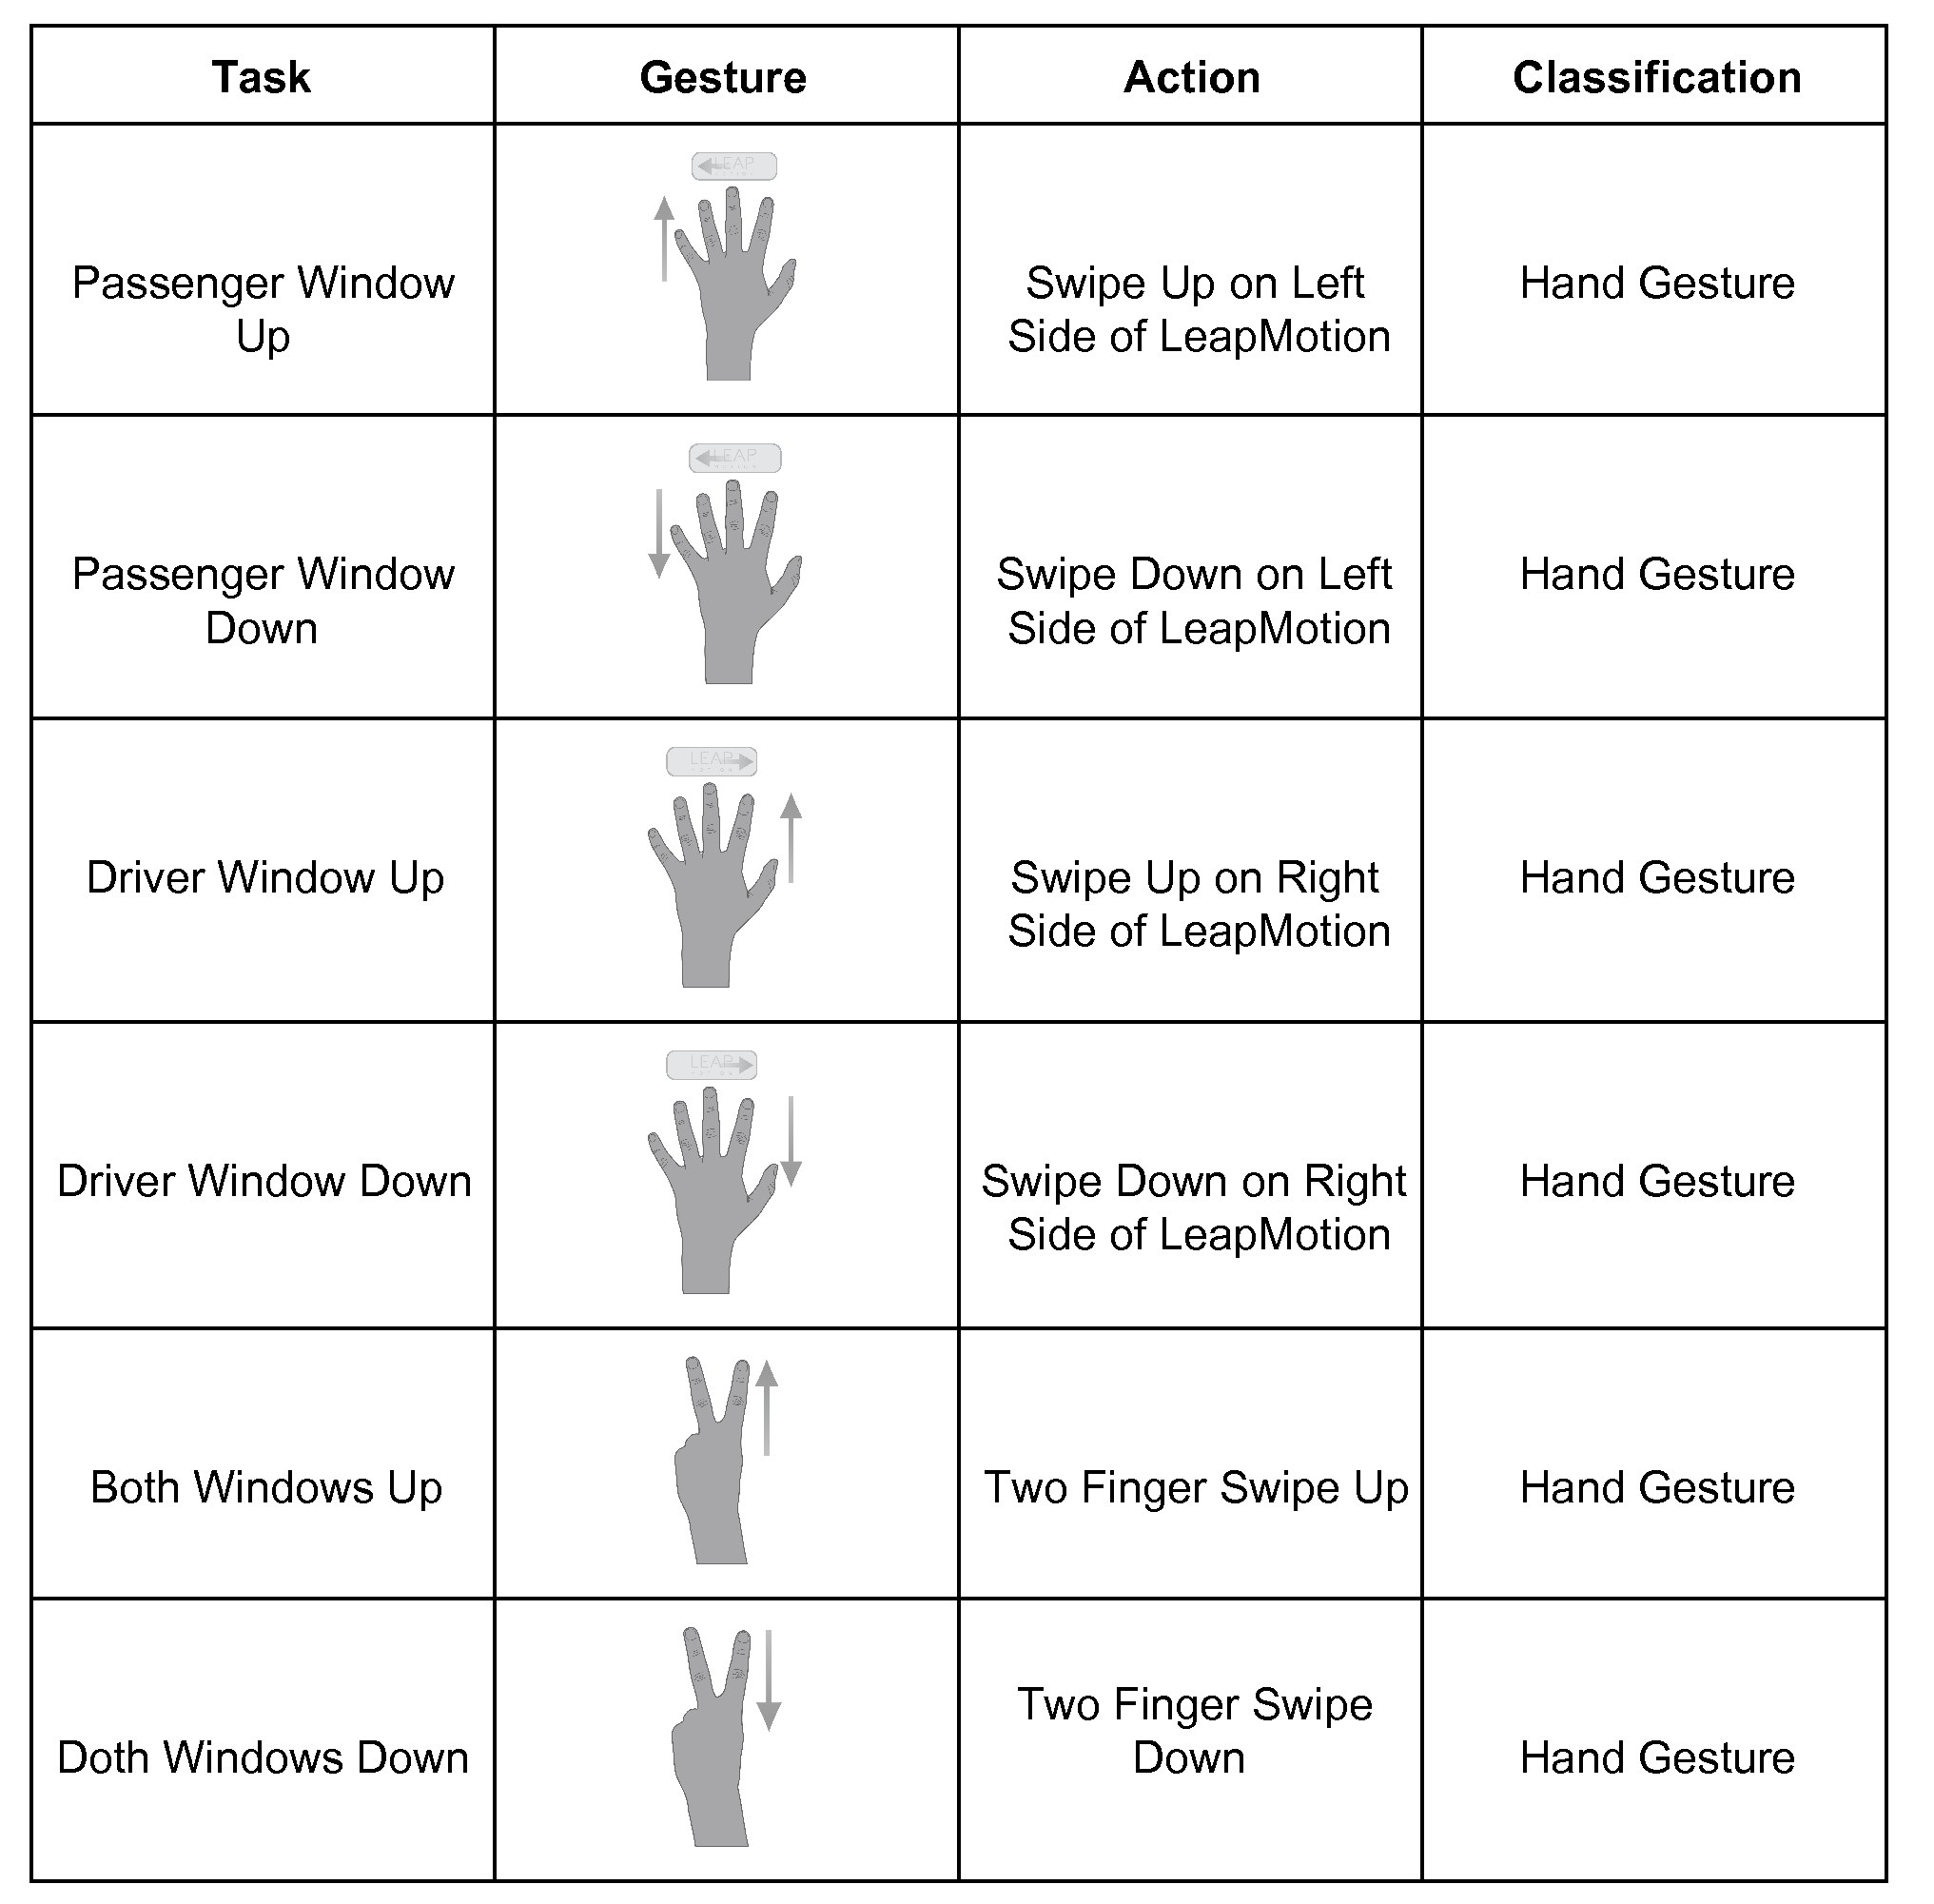
\includegraphics[width=6in]{images/LeapWindowGestures.png}
\label{fig:leapwindow}
\end{figure}
\newpage
\vspace{-3mm}

\subsection{Menu Hot-keys}
\vspace{-3mm}
One of the main objectives of the experiment was to discover if a streamlining process could exist for the main technological features within a vehicle. Regardless of where and what the user was currently on, they could carry out a specific gesture to jump directly to their desired location.  Conceptually this was presented to the participants as such:

\begin{table*}[!ht]
\hfill{}
\texttt{
\begin{tabular}{@{}p{-50mm}p{15mm}p{120mm}@{}}
& \textbf{Myself:} & "Imagine a scenario where you are currently on your GPS, following a route and you wish to change the album you are listening to. Instead of going back through previous menus, is there a gesture you can think of that will take you directly to music?" \\
\end{tabular}
\hfill{}
}
\end{table*}

This proved to be a challenging task and no common agreement existed between the participants. A number of methodologies were proposed by the users:

\begin{enumerate}

\item \textbf{Letter Recognition} -- Two people (15\%) suggested writing a letter associated with each feature within the vehicle. Although a novel idea, issues could arise if features share the same key letter or if the letter chosen for the feature does not resonate with the user – in such cases, the user may select the wrong option or forget the gesture completely, leading to frustration.

\item \textbf{Pre-determined Areas} -- Another two participants (23\%) constructed the idea of having a pre-defined area in the vehicle for each feature. Another interesting concept but has flaws, which can be best surmised in the following conversation with a user during the experiment:

\begin{table*}[!ht]
\hfill{}
\texttt{
\begin{tabular}{@{}p{-50mm}p{25mm}p{120mm}@{}}
& \textbf{Participant:} & "Say I have four areas, or however many areas are required – in the top left region, I have music. In the top right, I have GPS. And so on. That’s what I would do." \\\\
& \textbf{Myself:} & "Is that more of a free-motion gesture then? Will that not be quite a distraction as your hand is away from the wheel and gearstick for a period of time?" \\\\
& \textbf{Participant:} & "It doesn’t need to be a long period of time, just put that hand in that area quickly and it’ll switch to whatever feature." \\\\
& \textbf{Myself:} & "But say you are about to make a swipe gesture and instead it recognises your hand in that region and triggers that instead. Do you think hand accuracy is an important aspect or the gestures themselves?" \\\\
& \textbf{Participant:} & "Yeah...it’s difficult, because if you are too busy making sure your hand is detected, then you could end up being way more distracted while driving than before. But at the moment that is what I would suggest." \\
\end{tabular}
\hfill{}
}
\end{table*}

As specified in the non-functional requirements, the end user of \textbf{\textit{In-Car Gestural Interaction}} should not have to concern themselves with spacial coordination - it could lead to frustration, especially whilst driving, if the user is unable to place there hand in a recognised area. 
Furthermore, such gestures within the spatial area over the steering wheel could be misinterpreted by other drivers as signs to pull out or overtake, leading to accidents. The implication of certain gestures have to be considered, as mentioned in section blahblah\cite{}

\item \textbf{Finger Representation} -- Four users (31\%) proposed the idea of defining each area to a number, in a similar manner to hot-keys on a mobile phone. With the features assigned to a number, they can then be accessed by holding the corresponding number of fingers. Although this method requires recall - the driver needs to remember which number represents each finger – this appears to be an elegant solution. The issue of recall can be resolved through the UI design shown on the central console; this could either be a numbered grid or a list of options for example.

\item \textbf{Mimic Gestures} -- Five participants (38\%) suggested using the gesture that is the most synonymous for each task. For example, for accessing your phonebook, the participants picked up an imaginary phone with their hand. These gestures should be globally distinctive and are unlikely to hold any negative connotations in certain regions
\end{enumerate}

\subsubsection{Suggested Gestures}
\vspace{-3mm}
Disregarding the limitations of hardware, I would suggest following mimic gestures for switching between menu options.

If we take the first menu choice, Music, there are a number of mimicking gestures that could be associated to listening to music. The issue that arises however is that probably the most definable gesture, `holding headphones', requires two hands, making the gesture infeasible. The gestures never require both of the driver's hands, as specified in the functional requirements in section blah balh \cite{}, as it influences bad driving practices -- the driver’s primary responsibility is to drive and maintain constant control of the vehicle; having two handed gestures would encourage drivers to temporarily lose control of their car on purpose and could leap to more accidents attributed to distracted driving.

Instead, as figure blah blah \cite{} above shows, I would suggest a "pulling earlobe" to be the standardised gesture for music. As the five participants were aware of the dangers of driving without control, they all chose this simpler gesture to execute. Pulling on the earlobe is associated with hearing due to the charade gesture for "sounds like", these participants felt this was the best way to directly access music. as it is characteristic of the drivers desire (to access music) and is an identifiable gesture for hearing.

This, however, is not feasible using the LeapMotion due to its limited range. The alternative methods for gestures that are unattainable using the LeapMotion will be explored in Section blah blah.

\subsubsection{Gestures Defined for \textbf{\textit{In-Car Gestural Interaction}}}
\vspace{-3mm}
It is difficult to replicate mimicking gestures with the LeapMotion as it only tracks hand movements and not your full body, an alternative was required. 

Given that the majority of participants did not feel that there was a recognised symbol for every menu option, for the \textbf{\textit{In-Car Gestural Interaction Project}}, the most reliable way to allow users to switch between menus quickly was to determine their number of fingers detected over a set period of time. 

Given that four participants suggested this and the limitations of the LeapMotion, I felt that this was a feasible option. It may require a slight learning curve with users as it is not particularly intuitive, but once this is achieved, it should allow users to access the menu they desire, quickly and efficiently.

Furthermore, the driver will only have to remove their hand from the steering wheel for a brief period of time and as finger-counting is a small-scale gesture, the driver can quickly revert their hands to the wheel as required.

\subsection{Post Experiment Questionnaire}
\vspace{-3mm}
\section{Designing the User Interface}
\vspace{-3mm}
\subsection{Paper Prototype}
\vspace{-3mm}
\subsection{Storyboard}
\vspace{-3mm}

\chapter{Implementation}
\label{sec:implementation}
\vspace{-3mm}
\section{Creating the User Interface}
\vspace{-3mm}
\section{Finger Counting}
\vspace{-3mm}
\section{Gesture Recognition}
\vspace{-3mm}

\chapter{Evaluation}
\vspace{-3mm}
\section{Evaluation of Gestures and Mutlimodal Feedback}
\vspace{-3mm}
\section{Evaluation of User Interfaces}
\vspace{-3mm}
\section{Simulated Driving Evaluation}
\vspace{-3mm}

\chapter{Conclusion}
\label{sec:conc}
\vspace{-3mm}
\section{Summary of Project}
\vspace{-3mm}
\section{Future Work}
\vspace{-3mm}
\subsection{Refine Gesture Recognition}
\vspace{-3mm}
The LeapMotion simply isn't up to the task! developer features like an improved skeletal model of the hand that can better predict where fingers are even if it can’t see them—like when you curl your fingers into your palm—and defines individual fingers as specific finger types (like pinky and thumb, which can be helpful for, say, virtual keyboard apps). He says pinching and grabbing capabilities have also been improved. 

\subsection{Improve User Interface}
\vspace{-3mm}

\subsection{Determine Usability of Age Groups}
\vspace{-3mm}
If the technology was in the state that it could be tested in the field, would the reaction times between generations be significant or negligible?

Would older generations adopt the technology or sustain, continuing to use what they fell comfortable with?

\subsection{Measure Driver Coordination}
\vspace{-3mm}


\section*{Acknowledgments}
\label{sec:ack}
\vspace{-3mm}
We would like to thank Ian Miguel for his help in setting up the original CSPLib problem \cite{CSPLib},  and Mike Codish and Brendan McKay for pointing out errors in an earlier draft of this paper.


\bibliographystyle{plain}
\bibliography{bib}

\end{document}




